% !TEX program = xelatex
\documentclass[11pt]{article}


    \usepackage[breakable]{tcolorbox}
    \usepackage{parskip} % Stop auto-indenting (to mimic markdown behaviour)
    

    % Basic figure setup, for now with no caption control since it's done
    % automatically by Pandoc (which extracts ![](path) syntax from Markdown).
    \usepackage{graphicx}
    % Keep aspect ratio if custom image width or height is specified
    \setkeys{Gin}{keepaspectratio}
    % Maintain compatibility with old templates. Remove in nbconvert 6.0
    \let\Oldincludegraphics\includegraphics
    % Ensure that by default, figures have no caption (until we provide a
    % proper Figure object with a Caption API and a way to capture that
    % in the conversion process - todo).
    \usepackage{caption}
    \DeclareCaptionFormat{nocaption}{}
    \captionsetup{format=nocaption,aboveskip=0pt,belowskip=0pt}

    \usepackage{float}
    \floatplacement{figure}{H} % forces figures to be placed at the correct location
    \usepackage{xcolor} % Allow colors to be defined
    \usepackage{enumerate} % Needed for markdown enumerations to work
    \usepackage{geometry} % Used to adjust the document margins
    \usepackage{amsmath} % Equations
    \usepackage{amssymb} % Equations
    \usepackage{textcomp} % defines textquotesingle
    % Hack from http://tex.stackexchange.com/a/47451/13684:
    \AtBeginDocument{%
        \def\PYZsq{\textquotesingle}% Upright quotes in Pygmentized code
    }
    \usepackage{upquote} % Upright quotes for verbatim code
    \usepackage{eurosym} % defines \euro

    \usepackage{iftex}
    \ifPDFTeX
        \usepackage[T1]{fontenc}
        % Use plain [utf8]{inputenc}: utf8x conflicts with newunicodechar on
        % recent TeX Live (2024+), causing chars to silently not decode.
        \usepackage[utf8]{inputenc}
    \else
        \usepackage{fontspec}
        \usepackage{unicode-math}
    \fi

%, Unicode -> LaTeX mappings + emoji macros
% Loaded AFTER inputenc; declares EVERY non-ASCII char that appears in the body
% so plain [utf8]{inputenc} can decode it (utf8x's auto-mapping is gone).
\usepackage{newunicodechar}
\usepackage{pifont}
\providecommand{\cmark}{\texorpdfstring{{\color{green!60!black}\ding{51}}\,}{[+] }}
\providecommand{\xmark}{\texorpdfstring{{\color{red}\ding{55}}\,}{[-] }}
% (A few "Package newunicodechar Warning: Redefining Unicode character" lines
%  on the pdflatex path are harmless: T1 fontenc already maps a couple of
%  these to defaults and we override them with proper ensuremath versions.)
% Math symbols
\newunicodechar{≥}{\ensuremath{\geq}}
\newunicodechar{≤}{\ensuremath{\leq}}
\newunicodechar{≠}{\ensuremath{\neq}}
\newunicodechar{≈}{\ensuremath{\approx}}
\newunicodechar{↔}{\ensuremath{\leftrightarrow}}
\newunicodechar{→}{\ensuremath{\rightarrow}}
\newunicodechar{←}{\ensuremath{\leftarrow}}
\newunicodechar{²}{\ensuremath{^{2}}}
\newunicodechar{³}{\ensuremath{^{3}}}
\newunicodechar{·}{\ensuremath{\cdot}}
\newunicodechar{×}{\ensuremath{\times}}
% Greek letters that appear in body prose (not just math):
\newunicodechar{Δ}{\ensuremath{\Delta}}
\newunicodechar{α}{\ensuremath{\alpha}}
\newunicodechar{β}{\ensuremath{\beta}}
\newunicodechar{θ}{\ensuremath{\theta}}
\newunicodechar{ω}{\ensuremath{\omega}}

    \usepackage{fancyvrb} % verbatim replacement that allows latex
    \usepackage{grffile} % extends the file name processing of package graphics
                         % to support a larger range
    \makeatletter % fix for old versions of grffile with XeLaTeX
    \@ifpackagelater{grffile}{2019/11/01}
    {
      % Do nothing on new versions
    }
    {
      \def\Gread@@xetex#1{%
        \IfFileExists{"\Gin@base".bb}%
        {\Gread@eps{\Gin@base.bb}}%
        {\Gread@@xetex@aux#1}%
      }
    }
    \makeatother
    \usepackage[Export]{adjustbox} % Used to constrain images to a maximum size
    \adjustboxset{max size={0.9\linewidth}{0.9\paperheight}}

    % The hyperref package gives us a pdf with properly built
    % internal navigation ('pdf bookmarks' for the table of contents,
    % internal cross-reference links, web links for URLs, etc.)
    \usepackage{hyperref}
    % The default LaTeX title has an obnoxious amount of whitespace. By default,
    % titling removes some of it. It also provides customization options.
    \usepackage{titling}
    \usepackage{longtable} % longtable support required by pandoc >1.10
    \usepackage{booktabs}  % table support for pandoc > 1.12.2
    \usepackage{array}     % table support for pandoc >= 2.11.3
    \usepackage{calc}      % table minipage width calculation for pandoc >= 2.11.1
    \usepackage[inline]{enumitem} % IRkernel/repr support (it uses the enumerate* environment)
    \usepackage[normalem]{ulem} % ulem is needed to support strikethroughs (\sout)
                                % normalem makes italics be italics, not underlines
    \usepackage{soul}      % strikethrough (\st) support for pandoc >= 3.0.0
    \usepackage{mathrsfs}
    

    
    % Colors for the hyperref package
    \definecolor{urlcolor}{rgb}{0,.145,.698}
    \definecolor{linkcolor}{rgb}{.71,0.21,0.01}
    \definecolor{citecolor}{rgb}{.12,.54,.11}

    % ANSI colors
    \definecolor{ansi-black}{HTML}{3E424D}
    \definecolor{ansi-black-intense}{HTML}{282C36}
    \definecolor{ansi-red}{HTML}{E75C58}
    \definecolor{ansi-red-intense}{HTML}{B22B31}
    \definecolor{ansi-green}{HTML}{00A250}
    \definecolor{ansi-green-intense}{HTML}{007427}
    \definecolor{ansi-yellow}{HTML}{DDB62B}
    \definecolor{ansi-yellow-intense}{HTML}{B27D12}
    \definecolor{ansi-blue}{HTML}{208FFB}
    \definecolor{ansi-blue-intense}{HTML}{0065CA}
    \definecolor{ansi-magenta}{HTML}{D160C4}
    \definecolor{ansi-magenta-intense}{HTML}{A03196}
    \definecolor{ansi-cyan}{HTML}{60C6C8}
    \definecolor{ansi-cyan-intense}{HTML}{258F8F}
    \definecolor{ansi-white}{HTML}{C5C1B4}
    \definecolor{ansi-white-intense}{HTML}{A1A6B2}
    \definecolor{ansi-default-inverse-fg}{HTML}{FFFFFF}
    \definecolor{ansi-default-inverse-bg}{HTML}{000000}

    % common color for the border for error outputs.
    \definecolor{outerrorbackground}{HTML}{FFDFDF}

    % commands and environments needed by pandoc snippets
    % extracted from the output of `pandoc -s`
    \providecommand{\tightlist}{%
      \setlength{\itemsep}{0pt}\setlength{\parskip}{0pt}}
    \DefineVerbatimEnvironment{Highlighting}{Verbatim}{commandchars=\\\{\}}
    % Add ',fontsize=\small' for more characters per line
    \newenvironment{Shaded}{}{}
    \newcommand{\KeywordTok}[1]{\textcolor[rgb]{0.00,0.44,0.13}{\textbf{{#1}}}}
    \newcommand{\DataTypeTok}[1]{\textcolor[rgb]{0.56,0.13,0.00}{{#1}}}
    \newcommand{\DecValTok}[1]{\textcolor[rgb]{0.25,0.63,0.44}{{#1}}}
    \newcommand{\BaseNTok}[1]{\textcolor[rgb]{0.25,0.63,0.44}{{#1}}}
    \newcommand{\FloatTok}[1]{\textcolor[rgb]{0.25,0.63,0.44}{{#1}}}
    \newcommand{\CharTok}[1]{\textcolor[rgb]{0.25,0.44,0.63}{{#1}}}
    \newcommand{\StringTok}[1]{\textcolor[rgb]{0.25,0.44,0.63}{{#1}}}
    \newcommand{\CommentTok}[1]{\textcolor[rgb]{0.38,0.63,0.69}{\textit{{#1}}}}
    \newcommand{\OtherTok}[1]{\textcolor[rgb]{0.00,0.44,0.13}{{#1}}}
    \newcommand{\AlertTok}[1]{\textcolor[rgb]{1.00,0.00,0.00}{\textbf{{#1}}}}
    \newcommand{\FunctionTok}[1]{\textcolor[rgb]{0.02,0.16,0.49}{{#1}}}
    \newcommand{\RegionMarkerTok}[1]{{#1}}
    \newcommand{\ErrorTok}[1]{\textcolor[rgb]{1.00,0.00,0.00}{\textbf{{#1}}}}
    \newcommand{\NormalTok}[1]{{#1}}

    % Additional commands for more recent versions of Pandoc
    \newcommand{\ConstantTok}[1]{\textcolor[rgb]{0.53,0.00,0.00}{{#1}}}
    \newcommand{\SpecialCharTok}[1]{\textcolor[rgb]{0.25,0.44,0.63}{{#1}}}
    \newcommand{\VerbatimStringTok}[1]{\textcolor[rgb]{0.25,0.44,0.63}{{#1}}}
    \newcommand{\SpecialStringTok}[1]{\textcolor[rgb]{0.73,0.40,0.53}{{#1}}}
    \newcommand{\ImportTok}[1]{{#1}}
    \newcommand{\DocumentationTok}[1]{\textcolor[rgb]{0.73,0.13,0.13}{\textit{{#1}}}}
    \newcommand{\AnnotationTok}[1]{\textcolor[rgb]{0.38,0.63,0.69}{\textbf{\textit{{#1}}}}}
    \newcommand{\CommentVarTok}[1]{\textcolor[rgb]{0.38,0.63,0.69}{\textbf{\textit{{#1}}}}}
    \newcommand{\VariableTok}[1]{\textcolor[rgb]{0.10,0.09,0.49}{{#1}}}
    \newcommand{\ControlFlowTok}[1]{\textcolor[rgb]{0.00,0.44,0.13}{\textbf{{#1}}}}
    \newcommand{\OperatorTok}[1]{\textcolor[rgb]{0.40,0.40,0.40}{{#1}}}
    \newcommand{\BuiltInTok}[1]{{#1}}
    \newcommand{\ExtensionTok}[1]{{#1}}
    \newcommand{\PreprocessorTok}[1]{\textcolor[rgb]{0.74,0.48,0.00}{{#1}}}
    \newcommand{\AttributeTok}[1]{\textcolor[rgb]{0.49,0.56,0.16}{{#1}}}
    \newcommand{\InformationTok}[1]{\textcolor[rgb]{0.38,0.63,0.69}{\textbf{\textit{{#1}}}}}
    \newcommand{\WarningTok}[1]{\textcolor[rgb]{0.38,0.63,0.69}{\textbf{\textit{{#1}}}}}
    \makeatletter
    \newsavebox\pandoc@box
    \newcommand*\pandocbounded[1]{%
      \sbox\pandoc@box{#1}%
      % scaling factors for width and height
      \Gscale@div\@tempa\textheight{\dimexpr\ht\pandoc@box+\dp\pandoc@box\relax}%
      \Gscale@div\@tempb\linewidth{\wd\pandoc@box}%
      % select the smaller of both
      \ifdim\@tempb\p@<\@tempa\p@
        \let\@tempa\@tempb
      \fi
      % scaling accordingly (\@tempa < 1)
      \ifdim\@tempa\p@<\p@
        \scalebox{\@tempa}{\usebox\pandoc@box}%
      % scaling not needed, use as it is
      \else
        \usebox{\pandoc@box}%
      \fi
    }
    \makeatother

    % Define a nice break command that doesn't care if a line doesn't already
    % exist.
    \def\br{\hspace*{\fill} \\* }
    % Math Jax compatibility definitions
    \def\gt{>}
    \def\lt{<}
    \let\Oldtex\TeX
    \let\Oldlatex\LaTeX
    \renewcommand{\TeX}{\textrm{\Oldtex}}
    \renewcommand{\LaTeX}{\textrm{\Oldlatex}}
    % Document parameters
    % Document title
    \title{Bidirectional Totem-Pole PFC\\\large Control in abc and dq frames}
    \author{Kristian Skorpen}
    \date{\today}
    
    
    
    
    
    
    
% Pygments definitions
\makeatletter
\def\PY@reset{\let\PY@it=\relax \let\PY@bf=\relax%
    \let\PY@ul=\relax \let\PY@tc=\relax%
    \let\PY@bc=\relax \let\PY@ff=\relax}
\def\PY@tok#1{\csname PY@tok@#1\endcsname}
\def\PY@toks#1+{\ifx\relax#1\empty\else%
    \PY@tok{#1}\expandafter\PY@toks\fi}
\def\PY@do#1{\PY@bc{\PY@tc{\PY@ul{%
    \PY@it{\PY@bf{\PY@ff{#1}}}}}}}
\def\PY#1#2{\PY@reset\PY@toks#1+\relax+\PY@do{#2}}

\@namedef{PY@tok@w}{\def\PY@tc##1{\textcolor[rgb]{0.73,0.73,0.73}{##1}}}
\@namedef{PY@tok@c}{\let\PY@it=\textit\def\PY@tc##1{\textcolor[rgb]{0.24,0.48,0.48}{##1}}}
\@namedef{PY@tok@cp}{\def\PY@tc##1{\textcolor[rgb]{0.61,0.40,0.00}{##1}}}
\@namedef{PY@tok@k}{\let\PY@bf=\textbf\def\PY@tc##1{\textcolor[rgb]{0.00,0.50,0.00}{##1}}}
\@namedef{PY@tok@kp}{\def\PY@tc##1{\textcolor[rgb]{0.00,0.50,0.00}{##1}}}
\@namedef{PY@tok@kt}{\def\PY@tc##1{\textcolor[rgb]{0.69,0.00,0.25}{##1}}}
\@namedef{PY@tok@o}{\def\PY@tc##1{\textcolor[rgb]{0.40,0.40,0.40}{##1}}}
\@namedef{PY@tok@ow}{\let\PY@bf=\textbf\def\PY@tc##1{\textcolor[rgb]{0.67,0.13,1.00}{##1}}}
\@namedef{PY@tok@nb}{\def\PY@tc##1{\textcolor[rgb]{0.00,0.50,0.00}{##1}}}
\@namedef{PY@tok@nf}{\def\PY@tc##1{\textcolor[rgb]{0.00,0.00,1.00}{##1}}}
\@namedef{PY@tok@nc}{\let\PY@bf=\textbf\def\PY@tc##1{\textcolor[rgb]{0.00,0.00,1.00}{##1}}}
\@namedef{PY@tok@nn}{\let\PY@bf=\textbf\def\PY@tc##1{\textcolor[rgb]{0.00,0.00,1.00}{##1}}}
\@namedef{PY@tok@ne}{\let\PY@bf=\textbf\def\PY@tc##1{\textcolor[rgb]{0.80,0.25,0.22}{##1}}}
\@namedef{PY@tok@nv}{\def\PY@tc##1{\textcolor[rgb]{0.10,0.09,0.49}{##1}}}
\@namedef{PY@tok@no}{\def\PY@tc##1{\textcolor[rgb]{0.53,0.00,0.00}{##1}}}
\@namedef{PY@tok@nl}{\def\PY@tc##1{\textcolor[rgb]{0.46,0.46,0.00}{##1}}}
\@namedef{PY@tok@ni}{\let\PY@bf=\textbf\def\PY@tc##1{\textcolor[rgb]{0.44,0.44,0.44}{##1}}}
\@namedef{PY@tok@na}{\def\PY@tc##1{\textcolor[rgb]{0.41,0.47,0.13}{##1}}}
\@namedef{PY@tok@nt}{\let\PY@bf=\textbf\def\PY@tc##1{\textcolor[rgb]{0.00,0.50,0.00}{##1}}}
\@namedef{PY@tok@nd}{\def\PY@tc##1{\textcolor[rgb]{0.67,0.13,1.00}{##1}}}
\@namedef{PY@tok@s}{\def\PY@tc##1{\textcolor[rgb]{0.73,0.13,0.13}{##1}}}
\@namedef{PY@tok@sd}{\let\PY@it=\textit\def\PY@tc##1{\textcolor[rgb]{0.73,0.13,0.13}{##1}}}
\@namedef{PY@tok@si}{\let\PY@bf=\textbf\def\PY@tc##1{\textcolor[rgb]{0.64,0.35,0.47}{##1}}}
\@namedef{PY@tok@se}{\let\PY@bf=\textbf\def\PY@tc##1{\textcolor[rgb]{0.67,0.36,0.12}{##1}}}
\@namedef{PY@tok@sr}{\def\PY@tc##1{\textcolor[rgb]{0.64,0.35,0.47}{##1}}}
\@namedef{PY@tok@ss}{\def\PY@tc##1{\textcolor[rgb]{0.10,0.09,0.49}{##1}}}
\@namedef{PY@tok@sx}{\def\PY@tc##1{\textcolor[rgb]{0.00,0.50,0.00}{##1}}}
\@namedef{PY@tok@m}{\def\PY@tc##1{\textcolor[rgb]{0.40,0.40,0.40}{##1}}}
\@namedef{PY@tok@gh}{\let\PY@bf=\textbf\def\PY@tc##1{\textcolor[rgb]{0.00,0.00,0.50}{##1}}}
\@namedef{PY@tok@gu}{\let\PY@bf=\textbf\def\PY@tc##1{\textcolor[rgb]{0.50,0.00,0.50}{##1}}}
\@namedef{PY@tok@gd}{\def\PY@tc##1{\textcolor[rgb]{0.63,0.00,0.00}{##1}}}
\@namedef{PY@tok@gi}{\def\PY@tc##1{\textcolor[rgb]{0.00,0.52,0.00}{##1}}}
\@namedef{PY@tok@gr}{\def\PY@tc##1{\textcolor[rgb]{0.89,0.00,0.00}{##1}}}
\@namedef{PY@tok@ge}{\let\PY@it=\textit}
\@namedef{PY@tok@gs}{\let\PY@bf=\textbf}
\@namedef{PY@tok@ges}{\let\PY@bf=\textbf\let\PY@it=\textit}
\@namedef{PY@tok@gp}{\let\PY@bf=\textbf\def\PY@tc##1{\textcolor[rgb]{0.00,0.00,0.50}{##1}}}
\@namedef{PY@tok@go}{\def\PY@tc##1{\textcolor[rgb]{0.44,0.44,0.44}{##1}}}
\@namedef{PY@tok@gt}{\def\PY@tc##1{\textcolor[rgb]{0.00,0.27,0.87}{##1}}}
\@namedef{PY@tok@err}{\def\PY@bc##1{{\setlength{\fboxsep}{\string -\fboxrule}\fcolorbox[rgb]{1.00,0.00,0.00}{1,1,1}{\strut ##1}}}}
\@namedef{PY@tok@kc}{\let\PY@bf=\textbf\def\PY@tc##1{\textcolor[rgb]{0.00,0.50,0.00}{##1}}}
\@namedef{PY@tok@kd}{\let\PY@bf=\textbf\def\PY@tc##1{\textcolor[rgb]{0.00,0.50,0.00}{##1}}}
\@namedef{PY@tok@kn}{\let\PY@bf=\textbf\def\PY@tc##1{\textcolor[rgb]{0.00,0.50,0.00}{##1}}}
\@namedef{PY@tok@kr}{\let\PY@bf=\textbf\def\PY@tc##1{\textcolor[rgb]{0.00,0.50,0.00}{##1}}}
\@namedef{PY@tok@bp}{\def\PY@tc##1{\textcolor[rgb]{0.00,0.50,0.00}{##1}}}
\@namedef{PY@tok@fm}{\def\PY@tc##1{\textcolor[rgb]{0.00,0.00,1.00}{##1}}}
\@namedef{PY@tok@vc}{\def\PY@tc##1{\textcolor[rgb]{0.10,0.09,0.49}{##1}}}
\@namedef{PY@tok@vg}{\def\PY@tc##1{\textcolor[rgb]{0.10,0.09,0.49}{##1}}}
\@namedef{PY@tok@vi}{\def\PY@tc##1{\textcolor[rgb]{0.10,0.09,0.49}{##1}}}
\@namedef{PY@tok@vm}{\def\PY@tc##1{\textcolor[rgb]{0.10,0.09,0.49}{##1}}}
\@namedef{PY@tok@sa}{\def\PY@tc##1{\textcolor[rgb]{0.73,0.13,0.13}{##1}}}
\@namedef{PY@tok@sb}{\def\PY@tc##1{\textcolor[rgb]{0.73,0.13,0.13}{##1}}}
\@namedef{PY@tok@sc}{\def\PY@tc##1{\textcolor[rgb]{0.73,0.13,0.13}{##1}}}
\@namedef{PY@tok@dl}{\def\PY@tc##1{\textcolor[rgb]{0.73,0.13,0.13}{##1}}}
\@namedef{PY@tok@s2}{\def\PY@tc##1{\textcolor[rgb]{0.73,0.13,0.13}{##1}}}
\@namedef{PY@tok@sh}{\def\PY@tc##1{\textcolor[rgb]{0.73,0.13,0.13}{##1}}}
\@namedef{PY@tok@s1}{\def\PY@tc##1{\textcolor[rgb]{0.73,0.13,0.13}{##1}}}
\@namedef{PY@tok@mb}{\def\PY@tc##1{\textcolor[rgb]{0.40,0.40,0.40}{##1}}}
\@namedef{PY@tok@mf}{\def\PY@tc##1{\textcolor[rgb]{0.40,0.40,0.40}{##1}}}
\@namedef{PY@tok@mh}{\def\PY@tc##1{\textcolor[rgb]{0.40,0.40,0.40}{##1}}}
\@namedef{PY@tok@mi}{\def\PY@tc##1{\textcolor[rgb]{0.40,0.40,0.40}{##1}}}
\@namedef{PY@tok@il}{\def\PY@tc##1{\textcolor[rgb]{0.40,0.40,0.40}{##1}}}
\@namedef{PY@tok@mo}{\def\PY@tc##1{\textcolor[rgb]{0.40,0.40,0.40}{##1}}}
\@namedef{PY@tok@ch}{\let\PY@it=\textit\def\PY@tc##1{\textcolor[rgb]{0.24,0.48,0.48}{##1}}}
\@namedef{PY@tok@cm}{\let\PY@it=\textit\def\PY@tc##1{\textcolor[rgb]{0.24,0.48,0.48}{##1}}}
\@namedef{PY@tok@cpf}{\let\PY@it=\textit\def\PY@tc##1{\textcolor[rgb]{0.24,0.48,0.48}{##1}}}
\@namedef{PY@tok@c1}{\let\PY@it=\textit\def\PY@tc##1{\textcolor[rgb]{0.24,0.48,0.48}{##1}}}
\@namedef{PY@tok@cs}{\let\PY@it=\textit\def\PY@tc##1{\textcolor[rgb]{0.24,0.48,0.48}{##1}}}

\def\PYZbs{\char`\\}
\def\PYZus{\char`\_}
\def\PYZob{\char`\{}
\def\PYZcb{\char`\}}
\def\PYZca{\char`\^}
\def\PYZam{\char`\&}
\def\PYZlt{\char`\<}
\def\PYZgt{\char`\>}
\def\PYZsh{\char`\#}
\def\PYZpc{\char`\%}
\def\PYZdl{\char`\$}
\def\PYZhy{\char`\-}
\def\PYZsq{\char`\'}
\def\PYZdq{\char`\"}
\def\PYZti{\char`\~}
% for compatibility with earlier versions
\def\PYZat{@}
\def\PYZlb{[}
\def\PYZrb{]}
\makeatother


    % For linebreaks inside Verbatim environment from package fancyvrb.
    \makeatletter
        \newbox\Wrappedcontinuationbox
        \newbox\Wrappedvisiblespacebox
        \newcommand*\Wrappedvisiblespace {\textcolor{red}{\textvisiblespace}}
        \newcommand*\Wrappedcontinuationsymbol {\textcolor{red}{\llap{\tiny$\m@th\hookrightarrow$}}}
        \newcommand*\Wrappedcontinuationindent {3ex }
        \newcommand*\Wrappedafterbreak {\kern\Wrappedcontinuationindent\copy\Wrappedcontinuationbox}
        % Take advantage of the already applied Pygments mark-up to insert
        % potential linebreaks for TeX processing.
        %        {, <, #, %, $, ' and ": go to next line.
        %        _, }, ^, &, >, - and ~: stay at end of broken line.
        % Use of \textquotesingle for straight quote.
        \newcommand*\Wrappedbreaksatspecials {%
            \def\PYGZus{\discretionary{\char`\_}{\Wrappedafterbreak}{\char`\_}}%
            \def\PYGZob{\discretionary{}{\Wrappedafterbreak\char`\{}{\char`\{}}%
            \def\PYGZcb{\discretionary{\char`\}}{\Wrappedafterbreak}{\char`\}}}%
            \def\PYGZca{\discretionary{\char`\^}{\Wrappedafterbreak}{\char`\^}}%
            \def\PYGZam{\discretionary{\char`\&}{\Wrappedafterbreak}{\char`\&}}%
            \def\PYGZlt{\discretionary{}{\Wrappedafterbreak\char`\<}{\char`\<}}%
            \def\PYGZgt{\discretionary{\char`\>}{\Wrappedafterbreak}{\char`\>}}%
            \def\PYGZsh{\discretionary{}{\Wrappedafterbreak\char`\#}{\char`\#}}%
            \def\PYGZpc{\discretionary{}{\Wrappedafterbreak\char`\%}{\char`\%}}%
            \def\PYGZdl{\discretionary{}{\Wrappedafterbreak\char`\$}{\char`\$}}%
            \def\PYGZhy{\discretionary{\char`\-}{\Wrappedafterbreak}{\char`\-}}%
            \def\PYGZsq{\discretionary{}{\Wrappedafterbreak\textquotesingle}{\textquotesingle}}%
            \def\PYGZdq{\discretionary{}{\Wrappedafterbreak\char`\"}{\char`\"}}%
            \def\PYGZti{\discretionary{\char`\~}{\Wrappedafterbreak}{\char`\~}}%
        }
        % Some characters . , ; ? ! / are not pygmentized.
        % This macro makes them "active" and they will insert potential linebreaks
        \newcommand*\Wrappedbreaksatpunct {%
            \lccode`\~`\.\lowercase{\def~}{\discretionary{\hbox{\char`\.}}{\Wrappedafterbreak}{\hbox{\char`\.}}}%
            \lccode`\~`\,\lowercase{\def~}{\discretionary{\hbox{\char`\,}}{\Wrappedafterbreak}{\hbox{\char`\,}}}%
            \lccode`\~`\;\lowercase{\def~}{\discretionary{\hbox{\char`\;}}{\Wrappedafterbreak}{\hbox{\char`\;}}}%
            \lccode`\~`\:\lowercase{\def~}{\discretionary{\hbox{\char`\:}}{\Wrappedafterbreak}{\hbox{\char`\:}}}%
            \lccode`\~`\?\lowercase{\def~}{\discretionary{\hbox{\char`\?}}{\Wrappedafterbreak}{\hbox{\char`\?}}}%
            \lccode`\~`\!\lowercase{\def~}{\discretionary{\hbox{\char`\!}}{\Wrappedafterbreak}{\hbox{\char`\!}}}%
            \lccode`\~`\/\lowercase{\def~}{\discretionary{\hbox{\char`\/}}{\Wrappedafterbreak}{\hbox{\char`\/}}}%
            \catcode`\.\active
            \catcode`\,\active
            \catcode`\;\active
            \catcode`\:\active
            \catcode`\?\active
            \catcode`\!\active
            \catcode`\/\active
            \lccode`\~`\~
        }
    \makeatother

    \let\OriginalVerbatim=\Verbatim
    \makeatletter
    \renewcommand{\Verbatim}[1][1]{%
        %\parskip\z@skip
        \sbox\Wrappedcontinuationbox {\Wrappedcontinuationsymbol}%
        \sbox\Wrappedvisiblespacebox {\FV@SetupFont\Wrappedvisiblespace}%
        \def\FancyVerbFormatLine ##1{\hsize\linewidth
            \vtop{\raggedright\hyphenpenalty\z@\exhyphenpenalty\z@
                \doublehyphendemerits\z@\finalhyphendemerits\z@
                \strut ##1\strut}%
        }%
        % If the linebreak is at a space, the latter will be displayed as visible
        % space at end of first line, and a continuation symbol starts next line.
        % Stretch/shrink are however usually zero for typewriter font.
        \def\FV@Space {%
            \nobreak\hskip\z@ plus\fontdimen3\font minus\fontdimen4\font
            \discretionary{\copy\Wrappedvisiblespacebox}{\Wrappedafterbreak}
            {\kern\fontdimen2\font}%
        }%

        % Allow breaks at special characters using \PYG... macros.
        \Wrappedbreaksatspecials
        % Breaks at punctuation characters . , ; ? ! and / need catcode=\active
        \OriginalVerbatim[#1,codes*=\Wrappedbreaksatpunct]%
    }
    \makeatother

    % Exact colors from NB
    \definecolor{incolor}{HTML}{303F9F}
    \definecolor{outcolor}{HTML}{D84315}
    \definecolor{cellborder}{HTML}{CFCFCF}
    \definecolor{cellbackground}{HTML}{F7F7F7}

    % prompt
    \makeatletter
    \newcommand{\boxspacing}{\kern\kvtcb@left@rule\kern\kvtcb@boxsep}
    \makeatother
    \newcommand{\prompt}[4]{
        {\ttfamily\llap{{\color{#2}[#3]:\hspace{3pt}#4}}\vspace{-\baselineskip}}
    }
    

    
    % Prevent overflowing lines due to hard-to-break entities
    \sloppy
    % Setup hyperref package
    \hypersetup{
      breaklinks=true,  % so long urls are correctly broken across lines
      colorlinks=true,
      urlcolor=urlcolor,
      linkcolor=linkcolor,
      citecolor=citecolor,
      }
    % Slightly bigger margins than the latex defaults
    
    \geometry{verbose,tmargin=1in,bmargin=1in,lmargin=1in,rmargin=1in}
    
    

\begin{document}
\begin{center}
{\LARGE\bfseries Single-Phase Totem-Pole PFC}\\[4pt]
{\large Control in the abc frame}\\[8pt]
{\normalsize Kristian Skorpen}
\end{center}

    \hypertarget{introduction}{%
\section{Introduction}\label{introduction}}

    \begin{center}
    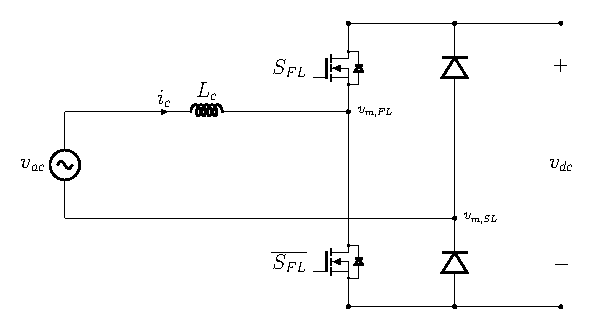
\includegraphics{figures/totem_pole_pfc_topology.pdf}
    \end{center}

    In this course we cover the \textbf{single-phase totem-pole PFC} and
how to control its input current (\(i_c\)) and active power drawn from
the grid. The totem-pole PFC is a rectifier: power flows from the AC
grid into the DC bus, and the control target is a sinusoidal input
current in phase with the grid voltage (unity power factor).

The course is built around control in the \textbf{stationary frame}
(abc), with derivations and runnable numerical examples in Python.

\begin{center}\rule{0.5\linewidth}{0.5pt}\end{center}

\hypertarget{learning-outcomes}{%
\subsection{Learning outcomes}\label{learning-outcomes}}

After completing this course you will be able to:

\begin{enumerate}
\def\labelenumi{\arabic{enumi}.}
\tightlist
\item
  Explain the topology of a single-phase totem-pole PFC and its
  fast-leg / slow-leg operation.
\item
  Derive the duty-cycle reference for a PWM modulator.
\item
  Implement a PI+feedforward current controller in the abc frame.
\item
  Implement an active power controller and a DC-link voltage
  controller, and decide which to use for a given application.
\end{enumerate}

\hypertarget{prerequisites}{%
\subsection{Prerequisites}\label{prerequisites}}

To take the course, I recommend a basic understanding of electronics,
math, and control theory. I expect that you understand, at a surface
level, how inductors and PI controllers work. However, you do not need
to understand how a totem-pole PFC works or how it is controlled. These
topics are covered in the course.

\hypertarget{notation-used-throughout}{%
\subsection{Notation (used throughout)}\label{notation-used-throughout}}

\begin{longtable}[]{@{}lll@{}}
\toprule
\begin{minipage}[b]{0.30\columnwidth}\raggedright
Symbol\strut
\end{minipage} & \begin{minipage}[b]{0.34\columnwidth}\raggedright
Meaning\strut
\end{minipage} & \begin{minipage}[b]{0.27\columnwidth}\raggedright
Units\strut
\end{minipage}\tabularnewline
\midrule
\endhead
\begin{minipage}[t]{0.30\columnwidth}\raggedright
\(v_{ac}, i_c\)\strut
\end{minipage} & \begin{minipage}[t]{0.34\columnwidth}\raggedright
Grid-side voltage and converter output (inductor) current,
time-domain\strut
\end{minipage} & \begin{minipage}[t]{0.27\columnwidth}\raggedright
V, A\strut
\end{minipage}\tabularnewline
\begin{minipage}[t]{0.30\columnwidth}\raggedright
\(V_{ac}, I_c\)\strut
\end{minipage} & \begin{minipage}[t]{0.34\columnwidth}\raggedright
\textbf{RMS} values of the same quantities (capital letters for
RMS)\strut
\end{minipage} & \begin{minipage}[t]{0.27\columnwidth}\raggedright
V, A\strut
\end{minipage}\tabularnewline
\begin{minipage}[t]{0.30\columnwidth}\raggedright
\(v_c\)\strut
\end{minipage} & \begin{minipage}[t]{0.34\columnwidth}\raggedright
Converter voltage (the PFC's controlled output)\strut
\end{minipage} & \begin{minipage}[t]{0.27\columnwidth}\raggedright
V\strut
\end{minipage}\tabularnewline
\begin{minipage}[t]{0.30\columnwidth}\raggedright
\(v_{dc}\)\strut
\end{minipage} & \begin{minipage}[t]{0.34\columnwidth}\raggedright
DC-link voltage\strut
\end{minipage} & \begin{minipage}[t]{0.27\columnwidth}\raggedright
V\strut
\end{minipage}\tabularnewline
\begin{minipage}[t]{0.30\columnwidth}\raggedright
\(L_c\)\strut
\end{minipage} & \begin{minipage}[t]{0.34\columnwidth}\raggedright
Output inductance\strut
\end{minipage} & \begin{minipage}[t]{0.27\columnwidth}\raggedright
H\strut
\end{minipage}\tabularnewline
\begin{minipage}[t]{0.30\columnwidth}\raggedright
\(\omega = 2\pi f_{ac}\)\strut
\end{minipage} & \begin{minipage}[t]{0.34\columnwidth}\raggedright
Grid angular frequency\strut
\end{minipage} & \begin{minipage}[t]{0.27\columnwidth}\raggedright
rad/s\strut
\end{minipage}\tabularnewline
\begin{minipage}[t]{0.30\columnwidth}\raggedright
\(\theta\)\strut
\end{minipage} & \begin{minipage}[t]{0.34\columnwidth}\raggedright
Grid voltage angle\strut
\end{minipage} & \begin{minipage}[t]{0.27\columnwidth}\raggedright
rad\strut
\end{minipage}\tabularnewline
\begin{minipage}[t]{0.30\columnwidth}\raggedright
\(\hat{\theta}\)\strut
\end{minipage} & \begin{minipage}[t]{0.34\columnwidth}\raggedright
PLL estimate of \(\theta\)\strut
\end{minipage} & \begin{minipage}[t]{0.27\columnwidth}\raggedright
rad\strut
\end{minipage}\tabularnewline
\begin{minipage}[t]{0.30\columnwidth}\raggedright
\(v_\alpha, v_\beta\)\strut
\end{minipage} & \begin{minipage}[t]{0.34\columnwidth}\raggedright
Clarke-transformed voltages (stationary)\strut
\end{minipage} & \begin{minipage}[t]{0.27\columnwidth}\raggedright
V\strut
\end{minipage}\tabularnewline
\begin{minipage}[t]{0.30\columnwidth}\raggedright
\(v_d, v_q, i_d, i_q\)\strut
\end{minipage} & \begin{minipage}[t]{0.34\columnwidth}\raggedright
Park-transformed voltages and currents (rotating)\strut
\end{minipage} & \begin{minipage}[t]{0.27\columnwidth}\raggedright
V, A\strut
\end{minipage}\tabularnewline
\begin{minipage}[t]{0.30\columnwidth}\raggedright
\(D_{FL}, S_{SL}\)\strut
\end{minipage} & \begin{minipage}[t]{0.34\columnwidth}\raggedright
Fast-leg duty cycle, slow-leg gate signal\strut
\end{minipage} & \begin{minipage}[t]{0.27\columnwidth}\raggedright
-, \{0,1\}\strut
\end{minipage}\tabularnewline
\begin{minipage}[t]{0.30\columnwidth}\raggedright
\(S_{FL}\)\strut
\end{minipage} & \begin{minipage}[t]{0.34\columnwidth}\raggedright
Fast-leg gate signal\strut
\end{minipage} & \begin{minipage}[t]{0.27\columnwidth}\raggedright
\{0,1\}\strut
\end{minipage}\tabularnewline
\begin{minipage}[t]{0.30\columnwidth}\raggedright
\(P, Q\)\strut
\end{minipage} & \begin{minipage}[t]{0.34\columnwidth}\raggedright
Active and reactive power (average)\strut
\end{minipage} & \begin{minipage}[t]{0.27\columnwidth}\raggedright
W, var\strut
\end{minipage}\tabularnewline
\bottomrule
\end{longtable}

Lower-case letters denote instantaneous time-domain quantities;
upper-case letters denote RMS values. Subscript \emph{ref} means
``commanded''; hat ( \(\hat{\cdot}\) ) means ``estimated''.

    \hypertarget{control-structure-in-the-abc-frame}{%
\subsubsection{Control Structure in the abc
frame}\label{control-structure-in-the-abc-frame}}

    \begin{center}
    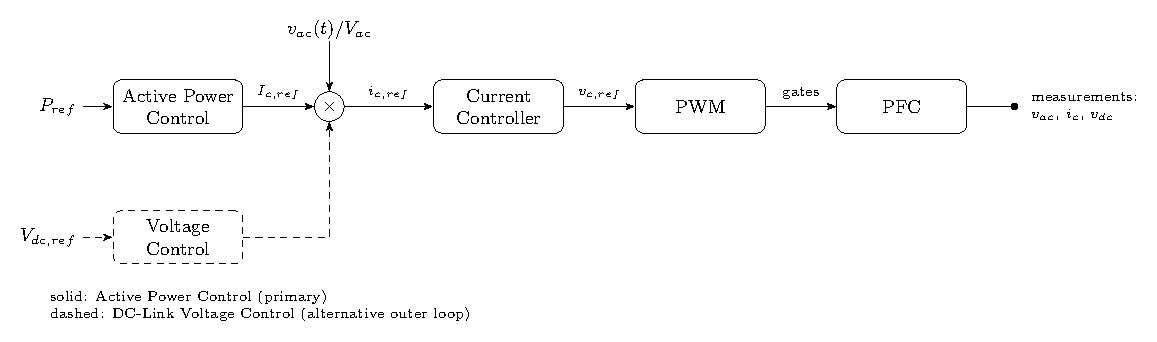
\includegraphics{figures/pfc_control_structure.pdf}
    \end{center}

    \clearpage
\setcounter{tocdepth}{3}
\tableofcontents
\newpage

\hypertarget{the-totem-pole-pfc}{%
\section{The Totem-Pole PFC}\label{the-totem-pole-pfc}}

    \hypertarget{topology}{%
\subsection{Topology}\label{topology}}

    A simplified model of a totem-pole PFC is shown in Figure 1. On
the left is a DC link, and on the right are an AC voltage source and an
inductor. In between, we have two switching legs. We use \emph{fast leg}
(FL) and \emph{slow leg} (SL) to refer to the left and right switching
legs, respectively. \(S_{FL}\) and \(S_{SL}\) are the gate signals for
the upper switches. Only one switch can be on at a time in each leg, as
indicated by the overline.

\begin{figure}
\centering
\begin{center}
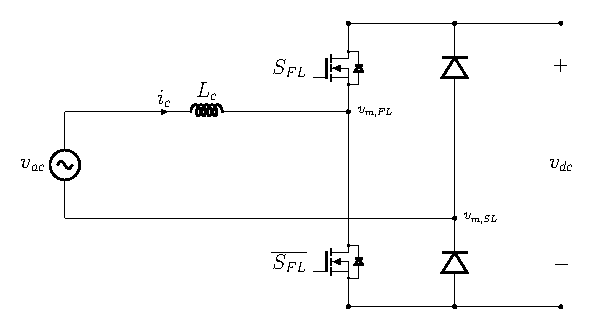
\includegraphics{figures/totem_pole_pfc_topology.pdf}
\end{center}
\caption{Figure 1: Totem-pole PFC}
\end{figure}

\emph{Figure 1: Totem-pole PFC}

The switching legs are called fast and slow because they switch at
different frequencies. The slow leg switches at twice the AC voltage
source's fundamental frequency. While the fast leg switches at a much
higher frequency. The fast-leg / slow-leg switching strategy is well
suited for a PFC rectifier and is a natural choice for a bidirectional
totem-pole PFC. If you design your own PFC, you will pick a
switching strategy to fit your goals (efficiency, EMI, device count).
The specific PWM choice does not change the current- or power-control
design that follows, this course is PWM-agnostic from the next
chapter onward. All chapters, except the PWM chapter, are relevant to
all types of PWM strategies. However, I will use the names ``fast leg''
and ``slow leg'' to distinguish between the two legs during switching.

Assumptions used throughout the rest of the course:

\begin{itemize}
\tightlist
\item
  Switches are ideal (zero on-resistance, instantaneous turn-on/off, no
  dead-time).
\item
  The DC-link voltage \(v_{dc}\) is constant and large enough that
  over-modulation does not occur (see PWM chapter for the explicit
  bound).
\item
  The output inductor \(L_c\) is linear (no core saturation, no
  equivalent series resistance).
\item
  The grid is modelled as a stiff sinusoidal voltage source
  \(v_{ac}(t) = \sqrt{2}\, V_{ac}\sin(\omega t)\).
\item
  No measurement or communication delay, every signal is available
  instantaneously.
\item
  Sampling time \(\Delta t\) is much shorter than the slowest controller
  time constant; discrete-time effects are discussed in the appendix.
\end{itemize}

These are idealisations. The \emph{When to use each method} chapter and
the appendix revisit them.

    \hypertarget{simplified-model-of-the-pfc}{%
\subsection{Simplified model of the
PFC}\label{simplified-model-of-the-pfc}}

    We can further simplify the model. If we look at \(v_{m,SL}\) in the
slow leg, when the upper switch is open (\(S_{SL}=0\)), \(v_{m,SL} = 0\)
and when it is closed (\(S_{SL}=1\)), \(v_{m,SL} = v_{dc}\). \(v_{dc}\)
is reference to ground.

\[
v_{m,SL} =
\begin{cases}
0, & S_{SL}=0 \\
v_{dc}, & S_{SL}=1
\end{cases}
\]

We can simplify this expression as:

\[
v_{m,SL} = S_{SL} \, v_{dc}
\]

And we can do the same for the fast leg:

\[
v_{m,FL} =
\begin{cases}
0, & S_{FL}=0 \\
v_{dc}, & S_{FL}=1
\end{cases}
\]

\[
v_{m,FL} = S_{FL} \, v_{dc}
\]

Because the fast leg and the slow leg can be modelled as voltages, we
can replace them with controlled voltage sources, as shown in Figure 2.
If we set the voltage reference (Ground) between the ac voltage
(\(v_{ac}\)) and the slow leg (\(v_{m,SL}\)), as shown in Figure 2. We
would get Figure 3, where \(v_c\) is the converter's output voltage.

\[
  v_c = v_{m, FL} - v_{m, SL}
\]

Ground is not shown explicitly: it is a reference and could be placed
anywhere.

\begin{figure}
\centering
\begin{center}
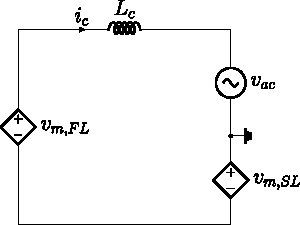
\includegraphics{figures/single-phase-to-inductor.pdf}
\end{center}
\caption{Figure 2: Fast-leg and slow-leg replaced by controlled voltage
sources. The output voltage is v\_c = v\_m,FL - v\_m,SL.}
\end{figure}

\emph{Figure 2: Fast-leg and slow-leg replaced by controlled voltage
sources. The output voltage is v\_c = v\_m,FL - v\_m,SL.}

\begin{figure}
\centering
\begin{center}
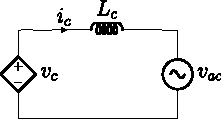
\includegraphics{figures/inductor.pdf}
\end{center}
\caption{Figure 3: Equivalent circuit used for the rest of the course
the PFC as a controlled voltage source v\_c in series with
inductor L\_c, feeding the grid voltage v\_ac.}
\end{figure}

\emph{Figure 3: Equivalent circuit used for the rest of the course
the PFC as a controlled voltage source v\_c in series with inductor
L\_c, feeding the grid voltage v\_ac.}

    From Figure 3 onwards, \emph{``the PFC''} means this equivalent
circuit: a controlled voltage source \(v_c\) in series with the output
inductor \(L_c\), feeding the stiff AC voltage \(v_{ac}\). Our job as
control designer is to pick \(v_c(t)\) so that the inductor current
\(i_c(t)\) follows a reference. The fast leg and the slow leg are the
physical actuators that realise \(v_c\).

    \hypertarget{control-structure}{%
\subsection{Control Structure}\label{control-structure}}

On a high level the control of a totem-pole PFC looks like this:

    \begin{center}
    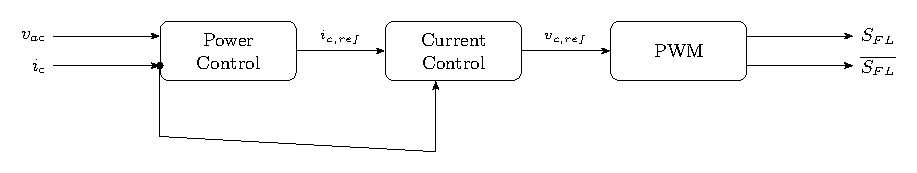
\includegraphics{figures/control_structure.pdf}
    \end{center}

    The controller is split into three blocks: \textbf{Power control},
\textbf{Current control}, and \textbf{PWM}. Each block operates on a
different timescale. PWM is an analog signal, meaning a continuous
signal, while the current controller is sampled in microseconds and the
power controller samples in milliseconds. The sampling times depend
heavily on application, but the sampling time of the current controller
is significantly lower than the sampling time for the power controller.
Each block can therefore be designed on the assumption that the block
below it has already settled, which is a standard and extremely
effective simplification.

First, we have the Power Control, which calculates the desired current
reference (\(i_{c,ref}\)) based on the measurements and the desired
Power. It is desired that the reference current (\(i_{c,ref}\)) changes
slowly in order not to introduce harmonics. Therefore, the Power
Controller can be sampled less often than the other block.

Then we have the Current Control, which calculates the reference voltage
(\(v_{c,ref}\)) for the PWM to achieve the desired current (\(i_c\)).

This controller does not control the DC-link voltage (\(v_{dc}\)).
Whether the PFC should control the DC-link voltage (\(v_{dc}\))
depends on the system around the PFC and the primary goals. We do
not go into detail on that here; if you want to control the dc-link
voltage (\(v_{dc}\)), you can replace the Power Control with a Voltage
Control. The input of the Voltage Controller would be the dc-link
voltage (\(v_{dc}\)) and the desired dc-link voltage, while the output
would be the reference current (\(i_{c,ref}\)), as for the Power
Controller. Whether you have a Power Controller or a Voltage Controller
does not affect the Current Controller or the PWM. The Voltage
Controller works well for unity power factor operations, and where
computational simplicity is important.

    \hypertarget{pwm-strategy}{%
\section{PWM Strategy}\label{pwm-strategy}}

    The PWM receives a reference voltage (\(v_{c, ref}\)) and generates gate
signals that drive the PFC. The reference voltage (\(v_{c, ref}\))
is given by the following equation as described above:

\[
v_{c, ref} = v_{m, FL} - v_{m, SL}
\]

    \hypertarget{gate-signal-derivation}{%
\subsection{Gate Signal Derivation}\label{gate-signal-derivation}}

    Remember that \(v_{m, FL}\) and \(v_{m, SL}\) are given by:

\[
v_{m, FL} = S_{FL} \, v_{dc}, \qquad v_{m, SL} = S_{SL} \, v_{dc}.
\]

Applying the fast-leg gate signal directly is computationally
prohibitive: at a 100 kHz switching frequency the outer controller would
need to resolve the gate state hundreds of thousands of times per
second. Instead we use an \textbf{average model} (also called
fundamental-frequency averaging): we compute a \emph{duty cycle}
\(D_{FL} \in [0,1]\), the average of \(S_{FL}\) over one switching
period, and let an analog comparator turn that into the actual gate
signal at the carrier frequency. The slow leg switches only twice per
grid period, so its gate signal \(S_{SL}\) is kept as-is.

The average-model replacement is

\[
v_{m,FL} = D_{FL} \, v_{dc}.
\]

Substituting into \(v_{c, ref} = v_{m, FL} - v_{m, SL}\):

\[
v_{c, ref} = D_{FL}\, v_{dc} - S_{SL}\, v_{dc}.
\]

The unknowns are \(D_{FL}\) (continuous, \([0,1]\)) and \(S_{SL}\)
(binary, \(\{0,1\}\)). Two cases:

\begin{itemize}
\tightlist
\item
  \textbf{If \(v_{c, ref} \leq 0\)}, choose \(S_{SL} = 0\) so
  \(v_{m,SL} = 0\). Then \(v_{c,ref} = D_{FL}\, v_{dc}\), but that would
  force \(D_{FL}\) negative when \(v_{c,ref}<0\), impossible. So
  instead we pick \(S_{SL} = 0\) when \(v_{c,ref} > 0\) and
  \(S_{SL} = 1\) when \(v_{c,ref} \leq 0\), which \emph{shifts} the
  fast-leg operating range into a feasible interval.
\item
  Solving the two-case system gives the compact form:
\end{itemize}

\[
S_{SL} = \begin{cases} 0 & \text{if } v_{c, ref} > 0 \\ 1 & \text{if } v_{c, ref} \leq 0 \end{cases},
\qquad
D_{FL} = S_{SL} + \frac{v_{c, ref}}{v_{dc}}.
\]

The equation is solvable only when \(|v_{c,ref}| \leq v_{dc}\). Outside
that range the PFC is \emph{over-modulated}: the converter simply
cannot produce the commanded voltage and the duty-cycle would have to
exceed \([0,1]\).

    The overall block diagram of the PWM would look like this:

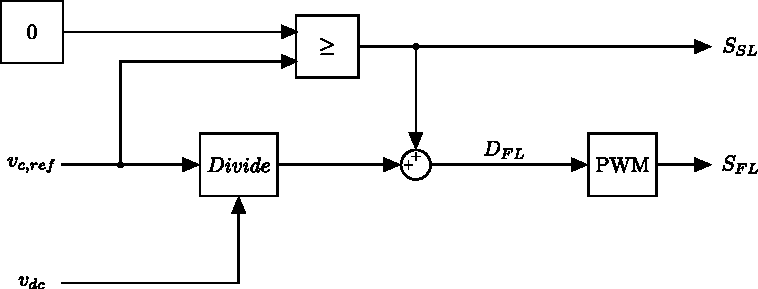
\includegraphics{figures/FastSlow_PWM_inv.pdf}

    \hypertarget{common-setup-run-this-block-once-then-every-numerical-example-reuses-it}{%
\subsection{Common setup (run this block once, then every numerical
example reuses
it)}\label{common-setup-run-this-block-once-then-every-numerical-example-reuses-it}}

All numerical examples below share imports, plotting helpers, and the
baseline grid parameters. Run the two cells in this section \textbf{once
at the start} of your session. Every later \emph{Numerical Example}
block will then work without re-declaring anything.

    \begin{tcolorbox}[breakable, size=fbox, boxrule=1pt, pad at break*=1mm,colback=cellbackground, colframe=cellborder]
\prompt{In}{incolor}{2}{\boxspacing}
\begin{Verbatim}[commandchars=\\\{\}]
\PY{k+kn}{import}\PY{+w}{ }\PY{n+nn}{numpy}\PY{+w}{ }\PY{k}{as}\PY{+w}{ }\PY{n+nn}{np}
\PY{k+kn}{import}\PY{+w}{ }\PY{n+nn}{importlib}
\PY{k+kn}{import}\PY{+w}{ }\PY{n+nn}{single\PYZus{}phase\PYZus{}inverter\PYZus{}functions}\PY{+w}{ }\PY{k}{as}\PY{+w}{ }\PY{n+nn}{inv\PYZus{}func}

\PY{n}{\PYZus{}} \PY{o}{=} \PY{n}{importlib}\PY{o}{.}\PY{n}{reload}\PY{p}{(}\PY{n}{inv\PYZus{}func}\PY{p}{)}
\end{Verbatim}
\end{tcolorbox}

    Common variables for all numerical examples:

    \begin{tcolorbox}[breakable, size=fbox, boxrule=1pt, pad at break*=1mm,colback=cellbackground, colframe=cellborder]
\prompt{In}{incolor}{3}{\boxspacing}
\begin{Verbatim}[commandchars=\\\{\}]
\PY{n}{Vac} \PY{o}{=} \PY{l+m+mi}{230}      \PY{c+c1}{\PYZsh{} RMS value of AC voltage}
\PY{n}{fac} \PY{o}{=} \PY{l+m+mi}{50}       \PY{c+c1}{\PYZsh{} Frequency of AC voltage}
\PY{n}{Vdc} \PY{o}{=} \PY{l+m+mi}{400}      \PY{c+c1}{\PYZsh{} Constant DC link voltage}
\PY{n}{Lc} \PY{o}{=} \PY{l+m+mf}{1e\PYZhy{}3}      \PY{c+c1}{\PYZsh{} Inductance}

\PY{c+c1}{\PYZsh{} Defining time}
\PY{n}{t\PYZus{}end} \PY{o}{=} \PY{l+m+mi}{1}\PY{o}{/}\PY{n}{fac}
\PY{n}{N} \PY{o}{=} \PY{l+m+mi}{1000} \PY{c+c1}{\PYZsh{} Number of samples}
\PY{n}{t} \PY{o}{=} \PY{n}{np}\PY{o}{.}\PY{n}{linspace}\PY{p}{(}\PY{l+m+mi}{0}\PY{p}{,} \PY{n}{t\PYZus{}end}\PY{p}{,} \PY{n}{N}\PY{p}{)}
\end{Verbatim}
\end{tcolorbox}

    \hypertarget{numerical-example}{%
\subsubsection{Numerical Example}\label{numerical-example}}

    \hypertarget{defining-parameters}{%
\paragraph{Defining Parameters}\label{defining-parameters}}

    \begin{tcolorbox}[breakable, size=fbox, boxrule=1pt, pad at break*=1mm,colback=cellbackground, colframe=cellborder]
\prompt{In}{incolor}{4}{\boxspacing}
\begin{Verbatim}[commandchars=\\\{\}]
\PY{c+c1}{\PYZsh{} Making a sine wave for vc\PYZus{}ref (Close to equivalent to Vac)}
\PY{n}{vc\PYZus{}ref}\PY{o}{=} \PY{n}{np}\PY{o}{.}\PY{n}{sqrt}\PY{p}{(}\PY{l+m+mi}{2}\PY{p}{)} \PY{o}{*} \PY{n}{Vac} \PY{o}{*} \PY{n}{np}\PY{o}{.}\PY{n}{sin}\PY{p}{(}\PY{l+m+mi}{2} \PY{o}{*} \PY{n}{np}\PY{o}{.}\PY{n}{pi} \PY{o}{*} \PY{n}{fac} \PY{o}{*} \PY{n}{t}\PY{p}{)} 
\end{Verbatim}
\end{tcolorbox}

    \hypertarget{calculating-pwm}{%
\paragraph{Calculating PWM}\label{calculating-pwm}}

    \begin{tcolorbox}[breakable, size=fbox, boxrule=1pt, pad at break*=1mm,colback=cellbackground, colframe=cellborder]
\prompt{In}{incolor}{5}{\boxspacing}
\begin{Verbatim}[commandchars=\\\{\}]
\PY{c+c1}{\PYZsh{} S\PYZus{}SL is 1 when v\PYZus{}c,ref \PYZlt{}= 0 and 0 when v\PYZus{}c,ref \PYZgt{} 0 (equation in the derivation above).}
\PY{c+c1}{\PYZsh{} Note: (vc\PYZus{}ref \PYZlt{} 0) gives the correct boundary up to the equal\PYZhy{}zero case, which is}
\PY{c+c1}{\PYZsh{} numerically measure\PYZhy{}zero for a sinusoidal vc\PYZus{}ref.}
\PY{n}{S\PYZus{}SL} \PY{o}{=} \PY{p}{(}\PY{n}{vc\PYZus{}ref} \PY{o}{\PYZlt{}}\PY{o}{=} \PY{l+m+mi}{0}\PY{p}{)}\PY{o}{.}\PY{n}{astype}\PY{p}{(}\PY{n+nb}{int}\PY{p}{)}

\PY{n}{D\PYZus{}FL} \PY{o}{=} \PY{n}{S\PYZus{}SL} \PY{o}{+} \PY{n}{vc\PYZus{}ref} \PY{o}{/} \PY{n}{Vdc}

\PY{n}{inv\PYZus{}func}\PY{o}{.}\PY{n}{plot\PYZus{}time\PYZus{}signals}\PY{p}{(}
    \PY{n}{t}\PY{p}{,}
    \PY{p}{[}
        \PY{p}{[}\PY{p}{[}\PY{n}{vc\PYZus{}ref}\PY{p}{,} \PY{l+s+s2}{\PYZdq{}}\PY{l+s+s2}{vc\PYZus{}ref}\PY{l+s+s2}{\PYZdq{}}\PY{p}{]}\PY{p}{,} \PY{p}{[}\PY{n}{Vdc}\PY{p}{,} \PY{l+s+s2}{\PYZdq{}}\PY{l+s+s2}{vdc}\PY{l+s+s2}{\PYZdq{}}\PY{p}{]}\PY{p}{]}\PY{p}{,}
        \PY{p}{[}\PY{p}{[}\PY{n}{S\PYZus{}SL}\PY{p}{,} \PY{l+s+s2}{\PYZdq{}}\PY{l+s+s2}{S\PYZus{}SL}\PY{l+s+s2}{\PYZdq{}}\PY{p}{]}\PY{p}{]}\PY{p}{,}
        \PY{p}{[}\PY{p}{[}\PY{n}{D\PYZus{}FL}\PY{p}{,} \PY{l+s+s2}{\PYZdq{}}\PY{l+s+s2}{D\PYZus{}FL}\PY{l+s+s2}{\PYZdq{}}\PY{p}{]}\PY{p}{]}\PY{p}{,}
    \PY{p}{]}
\PY{p}{)}
\end{Verbatim}
\end{tcolorbox}

    \begin{center}
    \adjustimage{max size={0.9\linewidth}{0.9\paperheight}}{single-phase-inverter_files/single-phase-inverter_32_0.png}
    \end{center}
    { \hspace*{\fill} \\}
    
    \hypertarget{control-in-abc-frame}{%
\section{Control in abc frame}\label{control-in-abc-frame}}

    The figure below gives an overview of how a single-phase bidirectional
totem-pole PFC can be controlled in the abc frame.

    \begin{center}
    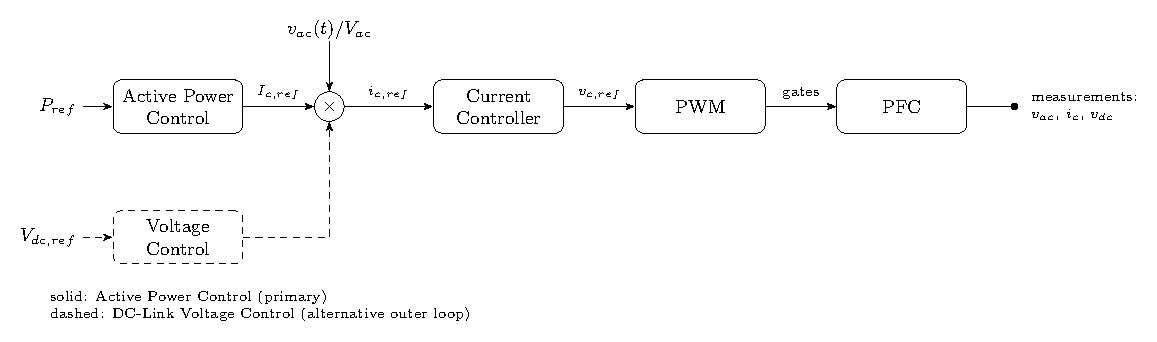
\includegraphics{figures/pfc_control_structure.pdf}
    \end{center}

    \hypertarget{current-control-in-abc-frame}{%
\subsection{Current Control in abc
Frame}\label{current-control-in-abc-frame}}

    \begin{figure}
\centering
\begin{center}
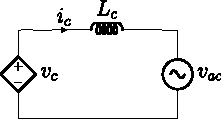
\includegraphics{figures/inductor.pdf}
\end{center}
\caption{Figure 3: Equivalent circuit used for the rest of the course
the PFC as a controlled voltage source v\_c in series with
inductor L\_c, feeding the grid voltage v\_ac.}
\end{figure}

\emph{Figure 3: Equivalent circuit used for the rest of the course
the PFC as a controlled voltage source v\_c in series with inductor
L\_c, feeding the grid voltage v\_ac.}

    The current we want to control is the output current, which is
equivalent to the inductor current (\(i_c\)). If we have a filter on the
output, it becomes more complicated, but the main principles are the
same. In this section, we will derive a current controller with PI and
feedforward.

    \hypertarget{derivation-of-the-reference-voltage}{%
\subsubsection{Derivation of the Reference
Voltage}\label{derivation-of-the-reference-voltage}}

    The inductor current depends on the voltage across the inductor. Writing
KVL around the loop in Figure 3:

\[
v_c \;-\; v_{L_c} \;-\; v_{ac} \;=\; 0
\qquad\Longrightarrow\qquad
v_c \;=\; v_{L_c} \;+\; v_{ac}.
\]

The inductor defining equation is

\[
v_{L_c} \;=\; L_c \, \frac{d i_c}{dt}.
\]

Combining the two:

\[
v_c \;=\; L_c \, \frac{d i_c}{dt} \;+\; v_{ac}.
\]

This is the \emph{plant} equation: it tells us what \(v_c\) we would
need if \(i_c\) followed its reference perfectly. Setting
\(v_c = v_{c,ref}\) and using a forward-Euler approximation
\(di_c/dt \approx (i_{c,ref}[k] - i_c[k-1]) / \Delta t\):

\[
v_{c,ref}[k] \;=\; \frac{L_c}{\Delta t}\, \big(i_{c,ref}[k] - i_c[k-1]\big) \;+\; v_{ac}[k].
\]

This is the \textbf{feedforward} reference: if the plant model were
perfect and we had no noise we would be done. The next section adds a PI
controller to cover for model mismatch and disturbances.

    \hypertarget{implementation-of-pi-controller}{%
\subsubsection{Implementation of PI
Controller}\label{implementation-of-pi-controller}}

    The feedforward equation above assumes a perfectly known inductor,
noise-free measurements, and zero delay. None of those hold in practice,
so we add a PI controller on the tracking error to handle the residual:

\[
v_{c, ref} \;=\; \underbrace{\frac{L_c}{\Delta t}\,(i_{c,ref} - i_c)}_{\text{discrete feedforward}} \;+\; \underbrace{v_{ac}}_{\text{grid feedforward}} \;+\; \underbrace{\mathrm{PI}(i_{c,ref} - i_c)}_{\text{correction}}.
\]

In many industrial implementations the discrete-feedforward term
\(L_c\,di_c/dt\) is \emph{dropped} because the numerical derivative of a
noisy current measurement amplifies that noise.

    \begin{center}
    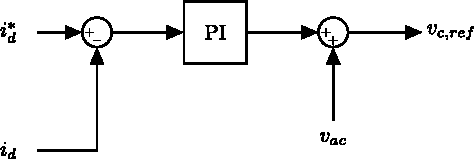
\includegraphics{figures/current_control_a.pdf}
    \end{center}

    \hypertarget{numerical-example-2}{%
\subsubsection{Numerical Example}\label{numerical-example-2}}

    \emph{(This example reuses the imports and grid parameters from the
\textbf{Common setup} section at the top. Run those cells first.)}

    \begin{tcolorbox}[breakable, size=fbox, boxrule=1pt, pad at break*=1mm,colback=cellbackground, colframe=cellborder]
\prompt{In}{incolor}{6}{\boxspacing}
\begin{Verbatim}[commandchars=\\\{\}]
\PY{c+c1}{\PYZsh{} Making a sine wave for vac}
\PY{n}{vac}\PY{o}{=} \PY{n}{np}\PY{o}{.}\PY{n}{sqrt}\PY{p}{(}\PY{l+m+mi}{2}\PY{p}{)} \PY{o}{*} \PY{n}{Vac} \PY{o}{*} \PY{n}{np}\PY{o}{.}\PY{n}{sin}\PY{p}{(}\PY{l+m+mi}{2} \PY{o}{*} \PY{n}{np}\PY{o}{.}\PY{n}{pi} \PY{o}{*} \PY{n}{fac} \PY{o}{*} \PY{n}{t}\PY{p}{)} 

\PY{c+c1}{\PYZsh{} Making a reference current}
\PY{n}{Iac} \PY{o}{=} \PY{l+m+mi}{15} \PY{c+c1}{\PYZsh{} RMS value of AC current}
\PY{n}{ic\PYZus{}ref} \PY{o}{=} \PY{n}{np}\PY{o}{.}\PY{n}{sqrt}\PY{p}{(}\PY{l+m+mi}{2}\PY{p}{)} \PY{o}{*} \PY{n}{Iac} \PY{o}{*} \PY{n}{np}\PY{o}{.}\PY{n}{sin}\PY{p}{(}\PY{l+m+mi}{2} \PY{o}{*} \PY{n}{np}\PY{o}{.}\PY{n}{pi} \PY{o}{*} \PY{n}{fac} \PY{o}{*} \PY{n}{t}\PY{p}{)}
\end{Verbatim}
\end{tcolorbox}

    \begin{tcolorbox}[breakable, size=fbox, boxrule=1pt, pad at break*=1mm,colback=cellbackground, colframe=cellborder]
\prompt{In}{incolor}{7}{\boxspacing}
\begin{Verbatim}[commandchars=\\\{\}]
\PY{c+c1}{\PYZsh{} \PYZhy{}\PYZhy{}\PYZhy{} Implementation (1 of 3): pure feedforward, no PI \PYZhy{}\PYZhy{}\PYZhy{}}
\PY{c+c1}{\PYZsh{} Plant + model are identical in this ideal example, so perfect tracking.}
\PY{c+c1}{\PYZsh{} Δt here is t[1]\PYZhy{}t[0]; ensure Δt \PYZlt{}\PYZlt{} 1 / switching frequency (Nyquist).}
\PY{n}{N\PYZus{}pwm} \PY{o}{=} \PY{n+nb}{len}\PY{p}{(}\PY{n}{t}\PY{p}{)}
\PY{n}{v\PYZus{}Lc} \PY{o}{=} \PY{n}{np}\PY{o}{.}\PY{n}{zeros}\PY{p}{(}\PY{n}{N\PYZus{}pwm}\PY{p}{)}
\PY{n}{ic}   \PY{o}{=} \PY{n}{np}\PY{o}{.}\PY{n}{zeros}\PY{p}{(}\PY{n}{N\PYZus{}pwm}\PY{p}{)}
\PY{n}{vc\PYZus{}ref} \PY{o}{=} \PY{n}{np}\PY{o}{.}\PY{n}{zeros}\PY{p}{(}\PY{n}{N\PYZus{}pwm}\PY{p}{)}
\PY{n}{ic}\PY{p}{[}\PY{l+m+mi}{0}\PY{p}{]} \PY{o}{=} \PY{l+m+mf}{0.0}  \PY{c+c1}{\PYZsh{} seed: assume zero initial current}

\PY{k}{for} \PY{n}{i} \PY{o+ow}{in} \PY{n+nb}{range}\PY{p}{(}\PY{l+m+mi}{1}\PY{p}{,} \PY{n}{N\PYZus{}pwm}\PY{p}{)}\PY{p}{:}
    \PY{n}{dt} \PY{o}{=} \PY{n}{t}\PY{p}{[}\PY{n}{i}\PY{p}{]} \PY{o}{\PYZhy{}} \PY{n}{t}\PY{p}{[}\PY{n}{i}\PY{o}{\PYZhy{}}\PY{l+m+mi}{1}\PY{p}{]}
    \PY{n}{v\PYZus{}Lc}\PY{p}{[}\PY{n}{i}\PY{p}{]} \PY{o}{=} \PY{n}{Lc} \PY{o}{/} \PY{n}{dt} \PY{o}{*} \PY{p}{(}\PY{n}{ic\PYZus{}ref}\PY{p}{[}\PY{n}{i}\PY{o}{\PYZhy{}}\PY{l+m+mi}{1}\PY{p}{]} \PY{o}{\PYZhy{}} \PY{n}{ic}\PY{p}{[}\PY{n}{i}\PY{o}{\PYZhy{}}\PY{l+m+mi}{1}\PY{p}{]}\PY{p}{)}
    \PY{n}{ic}\PY{p}{[}\PY{n}{i}\PY{p}{]}   \PY{o}{=} \PY{n}{ic}\PY{p}{[}\PY{n}{i}\PY{o}{\PYZhy{}}\PY{l+m+mi}{1}\PY{p}{]} \PY{o}{+} \PY{n}{v\PYZus{}Lc}\PY{p}{[}\PY{n}{i}\PY{p}{]} \PY{o}{*} \PY{n}{dt} \PY{o}{/} \PY{n}{Lc}

\PY{n}{vc\PYZus{}ref} \PY{o}{=} \PY{n}{v\PYZus{}Lc} \PY{o}{+} \PY{n}{vac}

\PY{n}{inv\PYZus{}func}\PY{o}{.}\PY{n}{plot\PYZus{}time\PYZus{}signals}\PY{p}{(}
    \PY{n}{t}\PY{p}{,}
    \PY{p}{[}
        \PY{p}{[}\PY{p}{[}\PY{n}{ic}\PY{p}{,} \PY{l+s+s2}{\PYZdq{}}\PY{l+s+s2}{ic}\PY{l+s+s2}{\PYZdq{}}\PY{p}{]}\PY{p}{,} \PY{p}{[}\PY{n}{ic\PYZus{}ref}\PY{p}{,} \PY{l+s+s2}{\PYZdq{}}\PY{l+s+s2}{ic\PYZus{}ref}\PY{l+s+s2}{\PYZdq{}}\PY{p}{,} \PY{l+s+s2}{\PYZdq{}}\PY{l+s+s2}{\PYZhy{}\PYZhy{}}\PY{l+s+s2}{\PYZdq{}}\PY{p}{]}\PY{p}{]}\PY{p}{,}
        \PY{p}{[}\PY{p}{[}\PY{n}{v\PYZus{}Lc}\PY{p}{,} \PY{l+s+s2}{\PYZdq{}}\PY{l+s+s2}{v\PYZus{}Lc}\PY{l+s+s2}{\PYZdq{}}\PY{p}{]}\PY{p}{]}\PY{p}{,}
        \PY{p}{[}\PY{p}{[}\PY{n}{vc\PYZus{}ref}\PY{p}{,} \PY{l+s+s2}{\PYZdq{}}\PY{l+s+s2}{vc\PYZus{}ref}\PY{l+s+s2}{\PYZdq{}}\PY{p}{]}\PY{p}{,} \PY{p}{[}\PY{n}{vac}\PY{p}{,} \PY{l+s+s2}{\PYZdq{}}\PY{l+s+s2}{vac}\PY{l+s+s2}{\PYZdq{}}\PY{p}{,} \PY{l+s+s2}{\PYZdq{}}\PY{l+s+s2}{\PYZhy{}\PYZhy{}}\PY{l+s+s2}{\PYZdq{}}\PY{p}{]}\PY{p}{]}\PY{p}{,}
    \PY{p}{]}\PY{p}{,}
    \PY{n}{height\PYZus{}per\PYZus{}plot}\PY{o}{=}\PY{l+m+mi}{2}
\PY{p}{)}
\end{Verbatim}
\end{tcolorbox}

    \begin{center}
    \adjustimage{max size={0.9\linewidth}{0.9\paperheight}}{single-phase-inverter_files/single-phase-inverter_48_0.png}
    \end{center}
    { \hspace*{\fill} \\}
    
    \begin{tcolorbox}[breakable, size=fbox, boxrule=1pt, pad at break*=1mm,colback=cellbackground, colframe=cellborder]
\prompt{In}{incolor}{ }{\boxspacing}
\begin{Verbatim}[commandchars=\\\{\}]
\PY{c+c1}{\PYZsh{} \PYZhy{}\PYZhy{}\PYZhy{} Implementation (2 of 3): pure PI, no feedforward \PYZhy{}\PYZhy{}\PYZhy{}}
\PY{c+c1}{\PYZsh{} No model term, only PI on the current error. Needs higher gains to track.}
\PY{n}{Kp\PYZus{}pi} \PY{o}{=} \PY{l+m+mf}{5.0}
\PY{n}{Ki\PYZus{}pi} \PY{o}{=} \PY{l+m+mf}{200.0}

\PY{n}{ic\PYZus{}pi}    \PY{o}{=} \PY{n}{np}\PY{o}{.}\PY{n}{zeros}\PY{p}{(}\PY{n}{N\PYZus{}pwm}\PY{p}{)}
\PY{n}{vc\PYZus{}ref\PYZus{}pi} \PY{o}{=} \PY{n}{np}\PY{o}{.}\PY{n}{zeros}\PY{p}{(}\PY{n}{N\PYZus{}pwm}\PY{p}{)}
\PY{n}{err\PYZus{}cum}  \PY{o}{=} \PY{l+m+mf}{0.0}

\PY{k}{for} \PY{n}{i} \PY{o+ow}{in} \PY{n+nb}{range}\PY{p}{(}\PY{l+m+mi}{1}\PY{p}{,} \PY{n}{N\PYZus{}pwm}\PY{p}{)}\PY{p}{:}
    \PY{n}{dt} \PY{o}{=} \PY{n}{t}\PY{p}{[}\PY{n}{i}\PY{p}{]} \PY{o}{\PYZhy{}} \PY{n}{t}\PY{p}{[}\PY{n}{i}\PY{o}{\PYZhy{}}\PY{l+m+mi}{1}\PY{p}{]}
    \PY{n}{err} \PY{o}{=} \PY{n}{ic\PYZus{}ref}\PY{p}{[}\PY{n}{i}\PY{o}{\PYZhy{}}\PY{l+m+mi}{1}\PY{p}{]} \PY{o}{\PYZhy{}} \PY{n}{ic\PYZus{}pi}\PY{p}{[}\PY{n}{i}\PY{o}{\PYZhy{}}\PY{l+m+mi}{1}\PY{p}{]}
    \PY{n}{err\PYZus{}cum} \PY{o}{+}\PY{o}{=} \PY{n}{err} \PY{o}{*} \PY{n}{dt}
    \PY{n}{v\PYZus{}cmd} \PY{o}{=} \PY{n}{Kp\PYZus{}pi} \PY{o}{*} \PY{n}{err} \PY{o}{+} \PY{n}{Ki\PYZus{}pi} \PY{o}{*} \PY{n}{err\PYZus{}cum}       \PY{c+c1}{\PYZsh{} PI output drives v\PYZus{}L}
    \PY{n}{ic\PYZus{}pi}\PY{p}{[}\PY{n}{i}\PY{p}{]} \PY{o}{=} \PY{n}{ic\PYZus{}pi}\PY{p}{[}\PY{n}{i}\PY{o}{\PYZhy{}}\PY{l+m+mi}{1}\PY{p}{]} \PY{o}{+} \PY{n}{v\PYZus{}cmd} \PY{o}{*} \PY{n}{dt} \PY{o}{/} \PY{n}{Lc}
    \PY{n}{vc\PYZus{}ref\PYZus{}pi}\PY{p}{[}\PY{n}{i}\PY{p}{]} \PY{o}{=} \PY{n}{v\PYZus{}cmd} \PY{o}{+} \PY{n}{vac}\PY{p}{[}\PY{n}{i}\PY{p}{]}

\PY{n}{inv\PYZus{}func}\PY{o}{.}\PY{n}{plot\PYZus{}time\PYZus{}signals}\PY{p}{(}
    \PY{n}{t}\PY{p}{,}
    \PY{p}{[}
        \PY{p}{[}\PY{p}{[}\PY{n}{ic\PYZus{}pi}\PY{p}{,} \PY{l+s+s2}{\PYZdq{}}\PY{l+s+s2}{ic (PI only)}\PY{l+s+s2}{\PYZdq{}}\PY{p}{]}\PY{p}{,} \PY{p}{[}\PY{n}{ic\PYZus{}ref}\PY{p}{,} \PY{l+s+s2}{\PYZdq{}}\PY{l+s+s2}{ic\PYZus{}ref}\PY{l+s+s2}{\PYZdq{}}\PY{p}{,} \PY{l+s+s2}{\PYZdq{}}\PY{l+s+s2}{\PYZhy{}\PYZhy{}}\PY{l+s+s2}{\PYZdq{}}\PY{p}{]}\PY{p}{]}\PY{p}{,}
        \PY{p}{[}\PY{p}{[}\PY{n}{vc\PYZus{}ref\PYZus{}pi}\PY{p}{,} \PY{l+s+s2}{\PYZdq{}}\PY{l+s+s2}{vc\PYZus{}ref}\PY{l+s+s2}{\PYZdq{}}\PY{p}{]}\PY{p}{,} \PY{p}{[}\PY{n}{vac}\PY{p}{,} \PY{l+s+s2}{\PYZdq{}}\PY{l+s+s2}{vac}\PY{l+s+s2}{\PYZdq{}}\PY{p}{,} \PY{l+s+s2}{\PYZdq{}}\PY{l+s+s2}{\PYZhy{}\PYZhy{}}\PY{l+s+s2}{\PYZdq{}}\PY{p}{]}\PY{p}{]}\PY{p}{,}
    \PY{p}{]}\PY{p}{,}
    \PY{n}{height\PYZus{}per\PYZus{}plot}\PY{o}{=}\PY{l+m+mi}{2}
\PY{p}{)}
\end{Verbatim}
\end{tcolorbox}

    \begin{tcolorbox}[breakable, size=fbox, boxrule=1pt, pad at break*=1mm,colback=cellbackground, colframe=cellborder]
\prompt{In}{incolor}{ }{\boxspacing}
\begin{Verbatim}[commandchars=\\\{\}]
\PY{c+c1}{\PYZsh{} \PYZhy{}\PYZhy{}\PYZhy{} Implementation (3 of 3): feedforward + PI (production pattern) \PYZhy{}\PYZhy{}\PYZhy{}}
\PY{c+c1}{\PYZsh{} Feedforward gives the bulk of the command; PI absorbs model error.}
\PY{n}{Kp\PYZus{}pi} \PY{o}{=} \PY{l+m+mf}{5.0}
\PY{n}{Ki\PYZus{}pi} \PY{o}{=} \PY{l+m+mf}{200.0}

\PY{n}{ic\PYZus{}ff\PYZus{}pi}    \PY{o}{=} \PY{n}{np}\PY{o}{.}\PY{n}{zeros}\PY{p}{(}\PY{n}{N\PYZus{}pwm}\PY{p}{)}
\PY{n}{vc\PYZus{}ref\PYZus{}ff\PYZus{}pi} \PY{o}{=} \PY{n}{np}\PY{o}{.}\PY{n}{zeros}\PY{p}{(}\PY{n}{N\PYZus{}pwm}\PY{p}{)}
\PY{n}{err\PYZus{}cum}     \PY{o}{=} \PY{l+m+mf}{0.0}

\PY{k}{for} \PY{n}{i} \PY{o+ow}{in} \PY{n+nb}{range}\PY{p}{(}\PY{l+m+mi}{1}\PY{p}{,} \PY{n}{N\PYZus{}pwm}\PY{p}{)}\PY{p}{:}
    \PY{n}{dt} \PY{o}{=} \PY{n}{t}\PY{p}{[}\PY{n}{i}\PY{p}{]} \PY{o}{\PYZhy{}} \PY{n}{t}\PY{p}{[}\PY{n}{i}\PY{o}{\PYZhy{}}\PY{l+m+mi}{1}\PY{p}{]}
    \PY{n}{err} \PY{o}{=} \PY{n}{ic\PYZus{}ref}\PY{p}{[}\PY{n}{i}\PY{o}{\PYZhy{}}\PY{l+m+mi}{1}\PY{p}{]} \PY{o}{\PYZhy{}} \PY{n}{ic\PYZus{}ff\PYZus{}pi}\PY{p}{[}\PY{n}{i}\PY{o}{\PYZhy{}}\PY{l+m+mi}{1}\PY{p}{]}
    \PY{n}{err\PYZus{}cum} \PY{o}{+}\PY{o}{=} \PY{n}{err} \PY{o}{*} \PY{n}{dt}
    \PY{n}{v\PYZus{}ff} \PY{o}{=} \PY{n}{Lc} \PY{o}{/} \PY{n}{dt} \PY{o}{*} \PY{p}{(}\PY{n}{ic\PYZus{}ref}\PY{p}{[}\PY{n}{i}\PY{p}{]} \PY{o}{\PYZhy{}} \PY{n}{ic\PYZus{}ff\PYZus{}pi}\PY{p}{[}\PY{n}{i}\PY{o}{\PYZhy{}}\PY{l+m+mi}{1}\PY{p}{]}\PY{p}{)}
    \PY{n}{v\PYZus{}pi} \PY{o}{=} \PY{n}{Kp\PYZus{}pi} \PY{o}{*} \PY{n}{err} \PY{o}{+} \PY{n}{Ki\PYZus{}pi} \PY{o}{*} \PY{n}{err\PYZus{}cum}
    \PY{n}{v\PYZus{}cmd} \PY{o}{=} \PY{n}{v\PYZus{}ff} \PY{o}{+} \PY{n}{v\PYZus{}pi}
    \PY{n}{ic\PYZus{}ff\PYZus{}pi}\PY{p}{[}\PY{n}{i}\PY{p}{]} \PY{o}{=} \PY{n}{ic\PYZus{}ff\PYZus{}pi}\PY{p}{[}\PY{n}{i}\PY{o}{\PYZhy{}}\PY{l+m+mi}{1}\PY{p}{]} \PY{o}{+} \PY{n}{v\PYZus{}cmd} \PY{o}{*} \PY{n}{dt} \PY{o}{/} \PY{n}{Lc}
    \PY{n}{vc\PYZus{}ref\PYZus{}ff\PYZus{}pi}\PY{p}{[}\PY{n}{i}\PY{p}{]} \PY{o}{=} \PY{n}{v\PYZus{}cmd} \PY{o}{+} \PY{n}{vac}\PY{p}{[}\PY{n}{i}\PY{p}{]}

\PY{n}{inv\PYZus{}func}\PY{o}{.}\PY{n}{plot\PYZus{}time\PYZus{}signals}\PY{p}{(}
    \PY{n}{t}\PY{p}{,}
    \PY{p}{[}
        \PY{p}{[}\PY{p}{[}\PY{n}{ic\PYZus{}ff\PYZus{}pi}\PY{p}{,} \PY{l+s+s2}{\PYZdq{}}\PY{l+s+s2}{ic (FF+PI)}\PY{l+s+s2}{\PYZdq{}}\PY{p}{]}\PY{p}{,} \PY{p}{[}\PY{n}{ic\PYZus{}ref}\PY{p}{,} \PY{l+s+s2}{\PYZdq{}}\PY{l+s+s2}{ic\PYZus{}ref}\PY{l+s+s2}{\PYZdq{}}\PY{p}{,} \PY{l+s+s2}{\PYZdq{}}\PY{l+s+s2}{\PYZhy{}\PYZhy{}}\PY{l+s+s2}{\PYZdq{}}\PY{p}{]}\PY{p}{]}\PY{p}{,}
        \PY{p}{[}\PY{p}{[}\PY{n}{vc\PYZus{}ref\PYZus{}ff\PYZus{}pi}\PY{p}{,} \PY{l+s+s2}{\PYZdq{}}\PY{l+s+s2}{vc\PYZus{}ref}\PY{l+s+s2}{\PYZdq{}}\PY{p}{]}\PY{p}{,} \PY{p}{[}\PY{n}{vac}\PY{p}{,} \PY{l+s+s2}{\PYZdq{}}\PY{l+s+s2}{vac}\PY{l+s+s2}{\PYZdq{}}\PY{p}{,} \PY{l+s+s2}{\PYZdq{}}\PY{l+s+s2}{\PYZhy{}\PYZhy{}}\PY{l+s+s2}{\PYZdq{}}\PY{p}{]}\PY{p}{]}\PY{p}{,}
    \PY{p}{]}\PY{p}{,}
    \PY{n}{height\PYZus{}per\PYZus{}plot}\PY{o}{=}\PY{l+m+mi}{2}
\PY{p}{)}
\end{Verbatim}
\end{tcolorbox}

    \hypertarget{pros-and-cons}{%
\subsubsection{Pros and Cons}\label{pros-and-cons}}

\hypertarget{pros}{%
\paragraph{\cmark{} Pros}\label{pros}}

\begin{itemize}
\tightlist
\item
  Simple implementation
\item
  No angle estimation (PLL)
\item
  Low computational cost
\end{itemize}

\hypertarget{cons}{%
\paragraph{\xmark{} Cons}\label{cons}}

\begin{itemize}
\tightlist
\item
  Control variables are sinusoidal
  \begin{itemize}
  \tightlist
  \item
    Harder to control
  \item
    Harder to analyze response
  \end{itemize}
\item
  Inductor voltage is not a part of feedforward
\end{itemize}

    \hypertarget{power-calculation-methods}{%
\subsection{Power Calculation Methods}\label{power-calculation-methods}}

    \begin{center}
    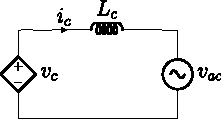
\includegraphics{figures/inductor.pdf}
    \end{center}

    \hypertarget{rms-based-definitions}{%
\subsubsection{RMS-based Definitions}\label{rms-based-definitions}}

    We want to measure and control the power delivered to the load/grid. The
apparent power is given by:

\[
    S = V_{ac, RMS} \; I_{c, RMS}
\]

The real value of S is the active power:

\[
    P = V_{ac, RMS} \; I_{c, RMS} \cos(\varphi)
\]

And the imaginary value is the reactive power: \[
    Q = V_{ac, RMS} \; I_{c, RMS} \sin(\varphi)
\]

The phase angle (\(\varphi\)) is the angle between the voltage and
current.

The power triangle is shown below, and from it we know that: \[
    S = \sqrt{P^2 + Q^2}
\]

    \begin{center}
    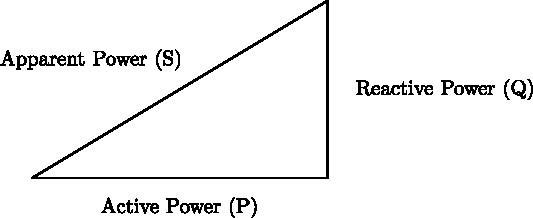
\includegraphics{figures/Power_Triangle.pdf}
    \end{center}

    For currents and voltages, capital letters denote RMS values, while
lowercase letters denote time-domain values. For example, \(V_{ac}\) is
the RMS value of the AC voltage, while \(v_{ac}\) is the time-domain
value of the AC voltage. We use this convention from now on. However,
this is only for currents and voltages. For example, P is given in the
time domain.

    \hypertarget{alternative-calculation-methods}{%
\subsubsection{Alternative calculation
Methods}\label{alternative-calculation-methods}}

    The problem with the calculation of \(P\) and \(Q\) shown above is that
we need to measure the voltage angle (\(\theta\)) to calculate
\(\varphi\). In a single-phase system, it is hard to measure the voltage
angle. Therefore, The alternative way to calculate \(P\) and \(Q\).

    \hypertarget{simple-method}{%
\paragraph{Simple method}\label{simple-method}}

    The instantaneous power is

\[
p(t) \;=\; v_{ac}(t)\, i_c(t).
\]

Both signals are sinusoidal, so \(p(t)\) contains a DC component (the
average power \(P\)) plus a ripple at twice the grid frequency. We want
the average:

\[
P \;=\; \langle v_{ac}\, i_c \rangle \;=\; \text{LPF}\big(v_{ac}(t)\, i_c(t)\big).
\]

This is the standard industry method. It needs only \(v_{ac}\) and
\(i_c\) plus a low-pass filter to extract the average. From now on
lowercase \(p\) means the instantaneous product and uppercase \(P\)
means its time-average.

For the reactive power \(Q\) we can use the power triangle:

\[
Q \;=\; \sqrt{S^2 - P^2}, \qquad S \;=\; V_{ac, RMS}\, I_{c, RMS}.
\]

\textbf{This gives the magnitude only; the sign is lost.} We don't know
whether it is positive or negative. However, you can find the sign of
\(Q\) by looking at the angle between the voltage and the current. If
the angle is positive (inductive), \(Q\) is positive, and if the angle
is negative (capacitive), \(Q\) is negative.

This way of calculating \(Q\) is not used in industry, but it is nice
to know.

    \hypertarget{advanced-method-for-deeper-understanding}{%
\paragraph{Advanced method (For Deeper
Understanding)}\label{advanced-method-for-deeper-understanding}}

    This method requires information about the voltage angle (\(\theta\)).
It gives good intuition for how P and Q behave, so we sketch it briefly;
it is not used in our controller. This method is inspired by the
synchronous-machine power-flow equations. It is not the one we use in
the controller, but understanding it is valuable.

Here are the formulas for P and Q:

\[
    P = \frac{V_c V_{ac}}{\omega L_c} \sin \delta
\]

\[
    Q = \frac{V_{ac}}{\omega L_c} ( V_c \cos \delta - V_{ac} )
\]

The power angle (\(\delta\)) is the angle between \(v_{c}\) and
\(v_{ac}\) and is given by:

\[
    \delta = \theta_{v_c} - \theta_{v_{ac}}
\]

If \(\delta\) is close to 0 and \(V_c\) is close to \(V_{ac}\). We have
the following properties:

\[
    \delta \approx 0 \text{ and } V_c \approx V_{ac}
\]

A change in \(\delta\) will result in a change in \(P\) and a small
change in \(Q\).

\[
    \text{If } \Delta \delta > 0 \text{ then:}
    \begin{cases}
    \Delta P > 0 \\
    \Delta Q \approx 0
    \end{cases}
\]

While a change in \(V_{c}\) will result in a small change in \(P\), a
change in \(Q\) will result.

\[
    \text{If } \Delta V_{c} > 0 \text{ then:}
    \begin{cases}
    \Delta P \approx 0 \\
    \Delta Q > 0
    \end{cases}
\]

For a totem-pole PFC, \(\delta\) is small and \(V_c\) is close to \(V_{ac}\).
This means that we can control \(P\) by controlling \(\delta\) and
control \(Q\) by controlling the magnitude of \(v_{c}\).

We will not use these relationships in the controller, but they provide
a good understanding of how \(P\) and \(Q\) are controlled, since that
is essentially how the controller works. However, grid-forming inverters
use these equations to control \(P\) and \(Q\).

    \hypertarget{numerical-example-for-deeper-understanding}{%
\subsubsection{Numerical Example (For deeper
understanding)}\label{numerical-example-for-deeper-understanding}}

    \emph{(This example reuses the imports and grid parameters from the
\textbf{Common setup} section at the top. Run those cells first.)}

    Here is a numerical example of how P and Q depend on the angle between
\(v_{c}\) and \(v_{ac}\) and the magnitude of \(v_{c}\). As explained in
the advanced method above. And we will use the simple method to
calculate P and Q.

    \begin{tcolorbox}[breakable, size=fbox, boxrule=1pt, pad at break*=1mm,colback=cellbackground, colframe=cellborder]
\prompt{In}{incolor}{8}{\boxspacing}
\begin{Verbatim}[commandchars=\\\{\}]
\PY{c+c1}{\PYZsh{} Defining time}
\PY{n}{periods} \PY{o}{=} \PY{l+m+mi}{2}
\PY{n}{t\PYZus{}end\PYZus{}long} \PY{o}{=} \PY{n}{periods}\PY{o}{/}\PY{n}{fac}
\PY{n}{N\PYZus{}long} \PY{o}{=} \PY{l+m+mi}{10000} \PY{c+c1}{\PYZsh{} Number of samples}
\PY{n}{t\PYZus{}long} \PY{o}{=} \PY{n}{np}\PY{o}{.}\PY{n}{linspace}\PY{p}{(}\PY{l+m+mi}{0}\PY{p}{,} \PY{n}{t\PYZus{}end\PYZus{}long}\PY{p}{,} \PY{n}{N\PYZus{}long}\PY{p}{)}

\PY{n}{N\PYZus{}period} \PY{o}{=} \PY{n}{N} \PY{o}{/} \PY{n}{periods}

\PY{c+c1}{\PYZsh{} Making a sine wave for vac}
\PY{n}{vac}\PY{o}{=} \PY{n}{np}\PY{o}{.}\PY{n}{sqrt}\PY{p}{(}\PY{l+m+mi}{2}\PY{p}{)} \PY{o}{*} \PY{n}{Vac} \PY{o}{*} \PY{n}{np}\PY{o}{.}\PY{n}{sin}\PY{p}{(}\PY{l+m+mi}{2} \PY{o}{*} \PY{n}{np}\PY{o}{.}\PY{n}{pi} \PY{o}{*} \PY{n}{fac} \PY{o}{*} \PY{n}{t\PYZus{}long}\PY{p}{)}
\end{Verbatim}
\end{tcolorbox}

    Increase Active Power -\textgreater{} Increase delta\_deg

Increase Reactive Power -\textgreater{} Increase mag\_scale

    \begin{tcolorbox}[breakable, size=fbox, boxrule=1pt, pad at break*=1mm,colback=cellbackground, colframe=cellborder]
\prompt{In}{incolor}{9}{\boxspacing}
\begin{Verbatim}[commandchars=\\\{\}]
\PY{n}{Lc\PYZus{}2} \PY{o}{=} \PY{l+m+mf}{5e\PYZhy{}3}      \PY{c+c1}{\PYZsh{} Inductance. It is deliberately oversized for illustration}
\PY{n}{delta\PYZus{}deg} \PY{o}{=} \PY{l+m+mi}{5}
\PY{n}{mag\PYZus{}scale} \PY{o}{=} \PY{l+m+mf}{1.0}

\PY{n}{inv\PYZus{}func}\PY{o}{.}\PY{n}{calc\PYZus{}and\PYZus{}plot\PYZus{}Power}\PY{p}{(}\PY{n}{t\PYZus{}long}\PY{p}{,} \PY{n}{vac}\PY{p}{,} \PY{n}{delta\PYZus{}deg}\PY{p}{,} \PY{n}{N\PYZus{}period}\PY{p}{,} \PY{n}{mag\PYZus{}scale}\PY{p}{,} \PY{n}{Lc\PYZus{}2}\PY{p}{)} \PY{c+c1}{\PYZsh{} This function can be found in the helper file}
\end{Verbatim}
\end{tcolorbox}

    \begin{Verbatim}[commandchars=\\\{\}]
S = 0.30 kVA
P\_avg = 0.30 kW
Q\_est = -0.00 kVAr
pf = 1.00
    \end{Verbatim}

    \begin{center}
    \adjustimage{max size={0.9\linewidth}{0.9\paperheight}}{single-phase-inverter_files/single-phase-inverter_70_1.png}
    \end{center}
    { \hspace*{\fill} \\}
    
    \hypertarget{pros-and-cons-power-calculation}{%
\subsubsection{Pros and Cons}\label{pros-and-cons-power-calculation}}

\hypertarget{pros-power-calculation}{%
\paragraph{\cmark{} Pros}\label{pros-power-calculation}}

\begin{itemize}
\tightlist
\item
  Simple implementation
\item
  No angle estimation (PLL)
\item
  Low computational cost
\end{itemize}

\hypertarget{cons-power-calculation}{%
\paragraph{\xmark{} Cons}\label{cons-power-calculation}}

\begin{itemize}
\tightlist
\item
  Contains 2ω ripple
\item
  Requires low-pass filtering (adds delay)
\item
  Reactive power estimation requires additional processing
\end{itemize}

    \hypertarget{pure-active-power-control}{%
\subsection{Pure Active Power Control}\label{pure-active-power-control}}

    Calculating the phase angle (\(\varphi\)) is not easily done for a
totem-pole PFC. A simple way to control active power with a
reactive-power reference of zero is as follows. This is the same control
method used by a \textbf{power-factor-correction rectifier (PFC)}: the
only target is unity power factor, i.e.~\(Q = 0\).

If the reactive power is zero, then the voltage and current are in phase
(\(\varphi = 0\)). The idea of this control method is that we assume
that the AC voltage (\(v_{ac}\)) is sinusoidal, and that the inductor
current (\(i_c\)) is controlled to have exactly the same waveform as the
AC voltage (\(v_{ac}\)). The desired inductor current is then obtained
by scaling the AC voltage to get the desired power:

\[
    i_{c,ref} = \frac{I_{c,ref}}{V_{ac}} v_{ac}
\]

Where \(I_{c,ref}\) is the RMS value of the reference current.

    \hypertarget{control-method}{%
\subsubsection{Control Method}\label{control-method}}

    The active power is found as described in the simple method above:

\[
    P = v_{ac} \, \, i_c
\]

The power has a ripple at twice the grid frequency. This is not a
problem for the PI controller provided its closed-loop bandwidth is well
below \(2\omega\). Concretely, at a 50 Hz grid the ripple sits at 100
Hz; a low-pass corner below \textasciitilde20 Hz rejects it by $\geq$14 dB.
In practice use an explicit low-pass on the measured \(P\) before the
PI, rather than relying on the PI to do the averaging.

When designing a PI controller, we want a linear relationship between
the input and the output. The average power should be constant in a
steady state, and the power is used to control the sinusoidal reference
current, so there is no linear relationship. Therefore, we should
decompose the reference current so that a PI controller calculates its
peak, which should be constant in the steady state. Now, we have a
linear relationship between the input and the output of the PI
controller.

    \hypertarget{implementation-of-pi-controller-2}{%
\subsubsection{Implementation of PI
Controller}\label{implementation-of-pi-controller-2}}

    \[
    I_{c,peak} = PI(P_{ref} - P) + I_{c, peak, FF}
\]

We can also add a feedforward term (\(I_{c, peak, FF}\)) to improve the
response. In an ideal case, we get:

\[
    I_{c,peak} = PI(P_{ref} - P) + \sqrt{2}\frac{P_{ref}}{V_{ac, RMS}}
\]

Units check: \([\text{W}]/[\text{V}] = [\text{A}]\), consistent with a
peak current. The \(\sqrt{2}\) converts RMS voltage to peak.

And then we oscillate the reference current peak to make it sinusoidal.

\[
    i_{c,ref} = I_{c,peak} \frac{v_{ac}}{\sqrt{2}V_{ac,RMS}}
\]

The Block diagram of the power control loop is shown in the figure
below.

\begin{center}
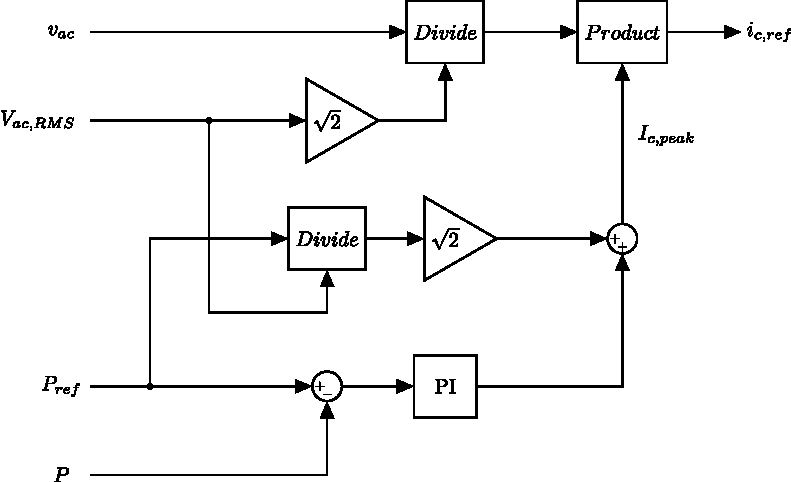
\includegraphics{figures/Pure_active_control.pdf}
\end{center}

    \hypertarget{numerical-example-3}{%
\subsubsection{Numerical Example}\label{numerical-example-3}}

    \emph{(This example reuses the imports and grid parameters from the
\textbf{Common setup} section at the top. Run those cells first.)}

    For this ideal model, the feedforward is close to ideal, so you won't
see the effect of the PI controller. Therefore, I have made two plots:
one with only a feedforward and one with only a PI controller.

    \hypertarget{only-feedforward}{%
\paragraph{Only Feedforward}\label{only-feedforward}}

    \begin{tcolorbox}[breakable, size=fbox, boxrule=1pt, pad at break*=1mm,colback=cellbackground, colframe=cellborder]
\prompt{In}{incolor}{10}{\boxspacing}
\begin{Verbatim}[commandchars=\\\{\}]
\PY{c+c1}{\PYZsh{} Defining time}
\PY{n}{t\PYZus{}end\PYZus{}long} \PY{o}{=} \PY{l+m+mi}{4}\PY{o}{/}\PY{n}{fac}
\PY{n}{N\PYZus{}long} \PY{o}{=} \PY{l+m+mi}{1000} \PY{c+c1}{\PYZsh{} Number of samples}
\PY{n}{t\PYZus{}long} \PY{o}{=} \PY{n}{np}\PY{o}{.}\PY{n}{linspace}\PY{p}{(}\PY{l+m+mi}{0}\PY{p}{,} \PY{n}{t\PYZus{}end\PYZus{}long}\PY{p}{,} \PY{n}{N\PYZus{}long}\PY{p}{)}

\PY{c+c1}{\PYZsh{} Making a sine wave for vac}
\PY{n}{vac}\PY{o}{=} \PY{n}{np}\PY{o}{.}\PY{n}{sqrt}\PY{p}{(}\PY{l+m+mi}{2}\PY{p}{)} \PY{o}{*} \PY{n}{Vac} \PY{o}{*} \PY{n}{np}\PY{o}{.}\PY{n}{sin}\PY{p}{(}\PY{l+m+mi}{2} \PY{o}{*} \PY{n}{np}\PY{o}{.}\PY{n}{pi} \PY{o}{*} \PY{n}{fac} \PY{o}{*} \PY{n}{t\PYZus{}long}\PY{p}{)} 

\PY{n}{P\PYZus{}ref} \PY{o}{=} \PY{l+m+mi}{3000} \PY{o}{*} \PY{n}{np}\PY{o}{.}\PY{n}{ones}\PY{p}{(}\PY{n}{N\PYZus{}long}\PY{p}{)}
\PY{n}{P\PYZus{}ref}\PY{p}{[}\PY{l+m+mi}{0}\PY{p}{:}\PY{n+nb}{int}\PY{p}{(}\PY{n}{N\PYZus{}long}\PY{o}{/}\PY{l+m+mi}{2}\PY{p}{)}\PY{p}{]} \PY{o}{=} \PY{n}{P\PYZus{}ref}\PY{p}{[}\PY{l+m+mi}{0}\PY{p}{:}\PY{n+nb}{int}\PY{p}{(}\PY{n}{N\PYZus{}long}\PY{o}{/}\PY{l+m+mi}{2}\PY{p}{)}\PY{p}{]} \PY{o}{*} \PY{n}{np}\PY{o}{.}\PY{n}{linspace}\PY{p}{(}\PY{l+m+mi}{0}\PY{p}{,} \PY{l+m+mi}{1}\PY{p}{,} \PY{n+nb}{int}\PY{p}{(}\PY{n}{N\PYZus{}long}\PY{o}{/}\PY{l+m+mi}{2}\PY{p}{)}\PY{p}{)}\PY{c+c1}{\PYZsh{} making a ramp}
\end{Verbatim}
\end{tcolorbox}

    \begin{tcolorbox}[breakable, size=fbox, boxrule=1pt, pad at break*=1mm,colback=cellbackground, colframe=cellborder]
\prompt{In}{incolor}{11}{\boxspacing}
\begin{Verbatim}[commandchars=\\\{\}]
\PY{n}{P} \PY{o}{=} \PY{n}{np}\PY{o}{.}\PY{n}{zeros}\PY{p}{(}\PY{n}{N\PYZus{}long}\PY{p}{)}
\PY{n}{ic\PYZus{}peak\PYZus{}ref} \PY{o}{=} \PY{n}{np}\PY{o}{.}\PY{n}{zeros}\PY{p}{(}\PY{n}{N\PYZus{}long}\PY{p}{)}
\PY{n}{ic\PYZus{}ref} \PY{o}{=} \PY{n}{np}\PY{o}{.}\PY{n}{zeros}\PY{p}{(}\PY{n}{N\PYZus{}long}\PY{p}{)}
\PY{n}{err\PYZus{}cum} \PY{o}{=} \PY{l+m+mi}{0}

    
\PY{n}{ic\PYZus{}peak\PYZus{}ref} \PY{o}{=} \PY{n}{np}\PY{o}{.}\PY{n}{sqrt}\PY{p}{(}\PY{l+m+mi}{2}\PY{p}{)} \PY{o}{*} \PY{n}{P\PYZus{}ref} \PY{o}{/} \PY{n}{Vac}

\PY{n}{ic\PYZus{}ref} \PY{o}{=} \PY{n}{ic\PYZus{}peak\PYZus{}ref} \PY{o}{*} \PY{n}{vac} \PY{o}{/} \PY{p}{(}\PY{n}{np}\PY{o}{.}\PY{n}{sqrt}\PY{p}{(}\PY{l+m+mi}{2}\PY{p}{)} \PY{o}{*} \PY{n}{Vac}\PY{p}{)}

\PY{n}{P} \PY{o}{=} \PY{n}{ic\PYZus{}ref} \PY{o}{*} \PY{n}{vac}


\PY{n}{inv\PYZus{}func}\PY{o}{.}\PY{n}{plot\PYZus{}time\PYZus{}signals}\PY{p}{(}
    \PY{n}{t\PYZus{}long}\PY{p}{,}
    \PY{p}{[}
        \PY{p}{[}\PY{p}{[}\PY{n}{P\PYZus{}ref}\PY{p}{,} \PY{l+s+s2}{\PYZdq{}}\PY{l+s+s2}{P\PYZus{}ref}\PY{l+s+s2}{\PYZdq{}}\PY{p}{]}\PY{p}{,} \PY{p}{[}\PY{n}{P}\PY{p}{,} \PY{l+s+s2}{\PYZdq{}}\PY{l+s+s2}{P}\PY{l+s+s2}{\PYZdq{}}\PY{p}{]}\PY{p}{]}\PY{p}{,}
        \PY{p}{[}\PY{p}{[}\PY{n}{ic\PYZus{}peak\PYZus{}ref}\PY{p}{,} \PY{l+s+s2}{\PYZdq{}}\PY{l+s+s2}{ic\PYZus{}peak\PYZus{}ref}\PY{l+s+s2}{\PYZdq{}}\PY{p}{]}\PY{p}{,} \PY{p}{[}\PY{n}{ic\PYZus{}ref}\PY{p}{,} \PY{l+s+s2}{\PYZdq{}}\PY{l+s+s2}{ic\PYZus{}ref}\PY{l+s+s2}{\PYZdq{}}\PY{p}{]}\PY{p}{]}\PY{p}{,}
    \PY{p}{]}\PY{p}{,}
    \PY{n}{height\PYZus{}per\PYZus{}plot}\PY{o}{=}\PY{l+m+mi}{2}
\PY{p}{)}
\end{Verbatim}
\end{tcolorbox}

    \begin{center}
    \adjustimage{max size={0.9\linewidth}{0.9\paperheight}}{single-phase-inverter_files/single-phase-inverter_85_0.png}
    \end{center}
    { \hspace*{\fill} \\}
    
    \hypertarget{pure-pi-controller}{%
\paragraph{Pure PI controller}\label{pure-pi-controller}}

    \begin{tcolorbox}[breakable, size=fbox, boxrule=1pt, pad at break*=1mm,colback=cellbackground, colframe=cellborder]
\prompt{In}{incolor}{12}{\boxspacing}
\begin{Verbatim}[commandchars=\\\{\}]
\PY{n}{t\PYZus{}end\PYZus{}long} \PY{o}{=} \PY{l+m+mi}{20}\PY{o}{/}\PY{n}{fac}
\PY{n}{N\PYZus{}long} \PY{o}{=} \PY{l+m+mi}{1000} \PY{c+c1}{\PYZsh{} Number of samples}
\PY{n}{t\PYZus{}long} \PY{o}{=} \PY{n}{np}\PY{o}{.}\PY{n}{linspace}\PY{p}{(}\PY{l+m+mi}{0}\PY{p}{,} \PY{n}{t\PYZus{}end\PYZus{}long}\PY{p}{,} \PY{n}{N\PYZus{}long}\PY{p}{)}

\PY{c+c1}{\PYZsh{} Making a sine wave for vac}
\PY{n}{vac}\PY{o}{=} \PY{n}{np}\PY{o}{.}\PY{n}{sqrt}\PY{p}{(}\PY{l+m+mi}{2}\PY{p}{)} \PY{o}{*} \PY{n}{Vac} \PY{o}{*} \PY{n}{np}\PY{o}{.}\PY{n}{sin}\PY{p}{(}\PY{l+m+mi}{2} \PY{o}{*} \PY{n}{np}\PY{o}{.}\PY{n}{pi} \PY{o}{*} \PY{n}{fac} \PY{o}{*} \PY{n}{t\PYZus{}long}\PY{p}{)} 

\PY{n}{P\PYZus{}ref} \PY{o}{=} \PY{l+m+mi}{3000} \PY{o}{*} \PY{n}{np}\PY{o}{.}\PY{n}{ones}\PY{p}{(}\PY{n}{N\PYZus{}long}\PY{p}{)}
\PY{n}{P\PYZus{}ref}\PY{p}{[}\PY{l+m+mi}{0}\PY{p}{:}\PY{n+nb}{int}\PY{p}{(}\PY{n}{N\PYZus{}long}\PY{o}{/}\PY{l+m+mi}{2}\PY{p}{)}\PY{p}{]} \PY{o}{=} \PY{n}{P\PYZus{}ref}\PY{p}{[}\PY{l+m+mi}{0}\PY{p}{:}\PY{n+nb}{int}\PY{p}{(}\PY{n}{N\PYZus{}long}\PY{o}{/}\PY{l+m+mi}{2}\PY{p}{)}\PY{p}{]} \PY{o}{*} \PY{n}{np}\PY{o}{.}\PY{n}{linspace}\PY{p}{(}\PY{l+m+mi}{0}\PY{p}{,} \PY{l+m+mi}{1}\PY{p}{,} \PY{n+nb}{int}\PY{p}{(}\PY{n}{N\PYZus{}long}\PY{o}{/}\PY{l+m+mi}{2}\PY{p}{)}\PY{p}{)}\PY{c+c1}{\PYZsh{} making a ramp}
\end{Verbatim}
\end{tcolorbox}

    \begin{tcolorbox}[breakable, size=fbox, boxrule=1pt, pad at break*=1mm,colback=cellbackground, colframe=cellborder]
\prompt{In}{incolor}{13}{\boxspacing}
\begin{Verbatim}[commandchars=\\\{\}]
\PY{n}{kp} \PY{o}{=} \PY{l+m+mf}{0.00001}
\PY{n}{ki} \PY{o}{=} \PY{l+m+mi}{1}

\PY{n}{P} \PY{o}{=} \PY{n}{np}\PY{o}{.}\PY{n}{zeros}\PY{p}{(}\PY{n}{N\PYZus{}long}\PY{p}{)}
\PY{n}{ic\PYZus{}peak\PYZus{}ref} \PY{o}{=} \PY{n}{np}\PY{o}{.}\PY{n}{zeros}\PY{p}{(}\PY{n}{N\PYZus{}long}\PY{p}{)}
\PY{n}{ic\PYZus{}ref} \PY{o}{=} \PY{n}{np}\PY{o}{.}\PY{n}{zeros}\PY{p}{(}\PY{n}{N\PYZus{}long}\PY{p}{)}
\PY{n}{err\PYZus{}cum} \PY{o}{=} \PY{l+m+mi}{0}

\PY{k}{for} \PY{n}{i} \PY{o+ow}{in} \PY{n+nb}{range}\PY{p}{(}\PY{l+m+mi}{1}\PY{p}{,} \PY{n}{N\PYZus{}long}\PY{p}{)}\PY{p}{:}
    \PY{n}{dt} \PY{o}{=} \PY{n}{t}\PY{p}{[}\PY{n}{i}\PY{p}{]} \PY{o}{\PYZhy{}} \PY{n}{t}\PY{p}{[}\PY{n}{i}\PY{o}{\PYZhy{}}\PY{l+m+mi}{1}\PY{p}{]}
    \PY{n}{err} \PY{o}{=} \PY{n}{P\PYZus{}ref}\PY{p}{[}\PY{n}{i}\PY{o}{\PYZhy{}}\PY{l+m+mi}{1}\PY{p}{]} \PY{o}{\PYZhy{}} \PY{n}{P}\PY{p}{[}\PY{n}{i}\PY{o}{\PYZhy{}}\PY{l+m+mi}{1}\PY{p}{]}
    \PY{n}{err\PYZus{}cum} \PY{o}{+}\PY{o}{=} \PY{n}{err} \PY{o}{*} \PY{n}{dt}
    
    \PY{n}{ic\PYZus{}peak\PYZus{}ref}\PY{p}{[}\PY{n}{i}\PY{p}{]} \PY{o}{=} \PY{n}{err} \PY{o}{*} \PY{n}{kp} \PY{o}{+} \PY{n}{err\PYZus{}cum} \PY{o}{*} \PY{n}{ki}

    \PY{n}{ic\PYZus{}ref}\PY{p}{[}\PY{n}{i}\PY{p}{]} \PY{o}{=} \PY{n}{ic\PYZus{}peak\PYZus{}ref}\PY{p}{[}\PY{n}{i}\PY{p}{]} \PY{o}{*} \PY{n}{vac}\PY{p}{[}\PY{n}{i}\PY{p}{]} \PY{o}{/} \PY{p}{(}\PY{n}{np}\PY{o}{.}\PY{n}{sqrt}\PY{p}{(}\PY{l+m+mi}{2}\PY{p}{)} \PY{o}{*} \PY{n}{Vac}\PY{p}{)}
    
    \PY{n}{P}\PY{p}{[}\PY{n}{i}\PY{p}{]} \PY{o}{=} \PY{n}{ic\PYZus{}ref}\PY{p}{[}\PY{n}{i}\PY{p}{]} \PY{o}{*} \PY{n}{vac}\PY{p}{[}\PY{n}{i}\PY{p}{]}


\PY{n}{inv\PYZus{}func}\PY{o}{.}\PY{n}{plot\PYZus{}time\PYZus{}signals}\PY{p}{(}
    \PY{n}{t\PYZus{}long}\PY{p}{,}
    \PY{p}{[}
        \PY{p}{[}\PY{p}{[}\PY{n}{P\PYZus{}ref}\PY{p}{,} \PY{l+s+s2}{\PYZdq{}}\PY{l+s+s2}{P\PYZus{}ref}\PY{l+s+s2}{\PYZdq{}}\PY{p}{]}\PY{p}{,} \PY{p}{[}\PY{n}{P}\PY{p}{,} \PY{l+s+s2}{\PYZdq{}}\PY{l+s+s2}{P}\PY{l+s+s2}{\PYZdq{}}\PY{p}{]}\PY{p}{]}\PY{p}{,}
        \PY{p}{[}\PY{p}{[}\PY{n}{ic\PYZus{}peak\PYZus{}ref}\PY{p}{,} \PY{l+s+s2}{\PYZdq{}}\PY{l+s+s2}{ic\PYZus{}peak\PYZus{}ref}\PY{l+s+s2}{\PYZdq{}}\PY{p}{]}\PY{p}{,} \PY{p}{[}\PY{n}{ic\PYZus{}ref}\PY{p}{,} \PY{l+s+s2}{\PYZdq{}}\PY{l+s+s2}{ic\PYZus{}ref}\PY{l+s+s2}{\PYZdq{}}\PY{p}{]}\PY{p}{]}\PY{p}{,}
    \PY{p}{]}\PY{p}{,}
    \PY{n}{height\PYZus{}per\PYZus{}plot}\PY{o}{=}\PY{l+m+mi}{2}
\PY{p}{)}
\end{Verbatim}
\end{tcolorbox}

    \begin{center}
    \adjustimage{max size={0.9\linewidth}{0.9\paperheight}}{single-phase-inverter_files/single-phase-inverter_88_0.png}
    \end{center}
    { \hspace*{\fill} \\}
    
    \hypertarget{pros-and-cons-2}{%
\subsubsection{Pros and Cons}\label{pros-and-cons-2}}

\hypertarget{pros-3}{%
\paragraph{\cmark{} Pros}\label{pros-3}}

\begin{itemize}
\tightlist
\item
  Simple implementation
\item
  No angle estimation (PLL)
\item
  Low computational cost
\item
  Suitable for unity power factor applications (PFC)
\end{itemize}

\hypertarget{cons-3}{%
\paragraph{\xmark{} Cons}\label{cons-3}}

\begin{itemize}
\tightlist
\item
  2ω ripple on power measurement
\item
  Limited flexibility for advanced grid support
\item
  Performance is strongly dependent on grid voltage quality
\item
  No Reactive Power Controller
\end{itemize}

    \hypertarget{dc-link-voltage-control}{%
\subsection{DC-Link Voltage Control}\label{dc-link-voltage-control}}

    The Pure Active Power Control in the previous section assumes you know
the desired active power \(P_{ref}\). In a typical PFC rectifier, the
primary goal is not a fixed power but a regulated DC-link voltage: the
downstream load draws whatever power it needs, and the PFC is expected
to draw exactly that much from the grid while keeping \(v_{dc}\)
constant.

The DC-link voltage controller is an outer loop that sits on top of the
Pure Active Power Control. Instead of commanding \(P_{ref}\) directly,
the user commands \(V_{dc,ref}\) and a PI controller generates the
current magnitude reference.

    \hypertarget{dc-link-control-method}{%
\subsubsection{Control Method}\label{dc-link-control-method}}

    The idea:

\begin{enumerate}
\def\labelenumi{\arabic{enumi}.}
\tightlist
\item
  Measure the DC-link voltage \(v_{dc}\).
\item
  Compute the error \(e_{v} = V_{dc,ref} - v_{dc}\).
\item
  A PI controller converts the error into a current magnitude reference
  \(I_{c,ref}\).
\item
  Shape the current reference using the grid-voltage waveform, as in
  Pure Active Power Control:
\end{enumerate}

\[
    i_{c,ref}(t) = \frac{I_{c,ref}}{V_{ac}}\, v_{ac}(t).
\]

\begin{enumerate}
\def\labelenumi{\arabic{enumi}.}
\setcounter{enumi}{4}
\tightlist
\item
  Feed \(i_{c,ref}(t)\) into the current controller, which generates
  the converter voltage reference \(v_{c,ref}\) as in Section~4.1.
\end{enumerate}

Because the DC-link capacitor is a slow storage element, the voltage
controller runs at a lower bandwidth than the current controller. This
bandwidth separation keeps the cascade stable without explicit
decoupling.

    \begin{center}
    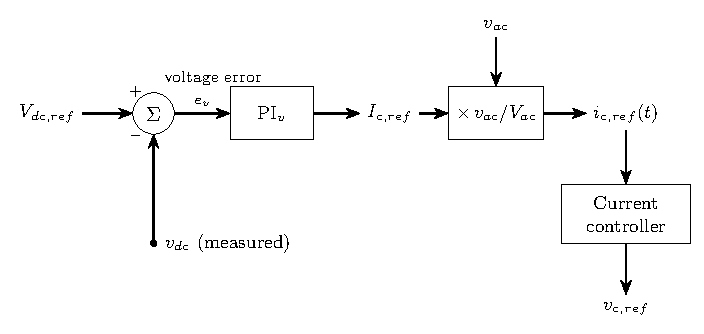
\includegraphics{figures/voltage_control_diagram.pdf}
    \end{center}

    \hypertarget{dc-link-pros-and-cons}{%
\subsubsection{Pros and Cons}\label{dc-link-pros-and-cons}}

\hypertarget{pros-dc-voltage}{%
\paragraph{\cmark{} Pros}\label{pros-dc-voltage}}

\begin{itemize}
\tightlist
\item
  Automatically matches power flow to the downstream load
\item
  Standard PFC rectifier configuration
\item
  No external power setpoint needed
\item
  Handles load transients through the outer voltage loop
\end{itemize}

\hypertarget{cons-dc-voltage}{%
\paragraph{\xmark{} Cons}\label{cons-dc-voltage}}

\begin{itemize}
\tightlist
\item
  Adds another control loop (slower outer loop to tune)
\item
  Requires a DC-link model (capacitor, load) for gain selection
\item
  2\(\omega\) ripple on the DC-link voltage couples back into
  \(I_{c,ref}\) unless aggressively filtered
\end{itemize}

    \hypertarget{comparison-of-control-methods}{%
\section{Comparison of Control
Methods}\label{comparison-of-control-methods}}

    This course presents two outer-loop options that sit above the same
current controller: \textbf{Pure Active Power Control} (you command
\(P_{ref}\)) and \textbf{DC-Link Voltage Control} (you command
\(V_{dc,ref}\)). Pick the one that matches what your higher-level
system already commands.

\textbf{Outer-loop target:}
\begin{itemize}
\tightlist
\item Active Power Control: user commands \(P_{ref}\) directly
\item DC-Link Voltage Control: user commands \(V_{dc,ref}\); power is
  whatever the downstream load draws
\end{itemize}

\textbf{Use case:}
\begin{itemize}
\tightlist
\item Active Power Control: the PFC sits inside a system that already
  computes a power setpoint (battery charger with an external charge
  controller, grid services with an external dispatch signal).
\item DC-Link Voltage Control: standalone PFC rectifier feeding a
  downstream DC load or an inverter; the DC bus must be regulated.
\end{itemize}

\textbf{Loop structure:}
\begin{itemize}
\tightlist
\item Active Power Control: single outer loop computing \(I_{c,ref}\)
  from a power setpoint.
\item DC-Link Voltage Control: extra outer loop that converts the
  DC-link error into \(I_{c,ref}\); the Active Power Control structure
  is nested inside.
\end{itemize}

\textbf{Tuning effort:}
\begin{itemize}
\tightlist
\item Active Power Control: one PI (current) plus a feedforward scale
  factor.
\item DC-Link Voltage Control: two PIs (current + voltage) with a
  bandwidth-separation requirement.
\end{itemize}

\textbf{2\(\omega\) ripple sensitivity:}
\begin{itemize}
\tightlist
\item Active Power Control: 2\(\omega\) ripple sits on the power
  estimate; filter bandwidth trades against response time.
\item DC-Link Voltage Control: 2\(\omega\) ripple sits on
  \(v_{dc}\); the voltage PI must be slow enough (or the filter
  aggressive enough) to ignore it, otherwise the ripple propagates
  into \(I_{c,ref}\) and distorts the grid current.
\end{itemize}

\end{document}
